\documentclass[10pt,twocolumn,letterpaper]{article}

\usepackage[review]{cvpr}
\usepackage{amsmath,amssymb}
\usepackage{booktabs}
\usepackage{graphicx}
\usepackage{multirow}
\usepackage{xcolor}
\usepackage[pagebackref,breaklinks,colorlinks]{hyperref}

\def\confName{CVPR}
\def\confYear{2026}
\def\paperID{0000}

\newcommand{\method}{CTF-GS}
\newcommand{\project}{RADIO-GS}
\newcommand{\radio}{C-RADIOv4-H}
\newcommand{\todo}[1]{\textcolor{red}{[#1]}}

\title{\method{}: Compact Teacher Feature Fields with View-to-Primitive Registration for Open-Vocabulary 3D Gaussian Scene Understanding}

\author{Anonymous Authors}
\date{}

\begin{document}
\maketitle

\begin{abstract}
We study whether dense vision-foundation features can be reconstructed as a
3D Gaussian scene representation and reused at novel views for open-vocabulary
scene understanding. Instead of training a scene-specific classifier or storing
raw high-dimensional features directly on every Gaussian, \method{} distills
frozen RADIO features into a Hybrid Gaussian Code Field (HGCF), reconstructs
teacher-space features with Compact-to-Teacher Reconstruction (CTR), and uses
View-Space Feature Alignment (VFA) plus Frozen Geometry-Head Consistency (FGC).
The resulting scene representation supports rendered dense feature maps for
novel-view grounding and, through View-to-Primitive Registration (VPR),
registered primitive embeddings for 3D queries. A label-free VPR-to-field
consistency stage can also transfer registered view evidence back into the
compact direct field. On LERF-OVS, the current frozen \project{} package reaches
0.8712 macro localization accuracy and 0.5243
calibrated macro mIoU across four scenes. On the VALA/OpenGaFF eight-scene
ScanNet direct point-query protocol, a conservative Gaussian-index readout
reaches 0.3583, 0.3618, and 0.4367 mIoU on the 19-, 15-, and 10-class splits;
the strongest DINO-CV contextual kNN point readout with label-free scene-mean
calibration further improves them to 0.3704, 0.3771, and 0.4585. An
OpenGaussian-style direct 3D object-selection evaluation shows that a
rendered-feature-to-primitive registration readout with a fixed global
softmax-score threshold, a 0.5\% selection floor, a 1.8\% selection cap, and
GT-free RGB boundary snap reaches 0.4801 macro mIoU and 0.6760 macro
Acc@0.25. With a frozen official SAM3 box-prompt readout, the compact direct
field reaches 0.5705 macro mIoU and 0.6835 Acc@0.25 under a fixed global
threshold; the scene-locked diagnostic upper bound reaches 0.5972/0.7009. For context, the raw Gaussian-center
diagnostic reaches only 0.012/0.009 under the fixed top-2\% selector used in
the VPR sweep and 0.0804/0.0932 under an earlier top-10\% selector; under the
same threshold-sweep diagnostic protocol, confidence-weighted VPR-to-field
consistency lifts the direct Gaussian-center readout from 0.0458/0.0707 to
0.4363/0.6191. These results
support the central claim that 3D Gaussian scenes can serve as reusable
foundation-feature memories across rendered-view and registered primitive-level
readouts, while clarifying that raw Gaussian-center readout is weak and Waldo
Kitchen remains a difficult object-fragmentation case.
\end{abstract}

\section{Introduction}

Vision foundation models expose dense features that are useful for recognition,
localization, segmentation, and geometric reasoning. However, most 3D scene
representations still optimize either RGB appearance or task-specific labels. In
open-vocabulary 3D understanding, this creates a gap: the strongest 2D feature
extractors are available at training images, but a deployed 3D scene must answer
queries from novel views.

\method{} targets this gap by reconstructing teacher foundation features inside a
3D Gaussian scene. Our goal is not to train a new per-scene language classifier.
Instead, we ask whether a scene representation can support two complementary
interfaces from the same compact field: dense novel-view feature maps for
rendered open-vocabulary localization, and registered primitive/point-level
features for direct 3D selection or semantic querying. This
feature-reconstruction framing differs from
methods that attach only a final language code to a radiance field or optimize a
single downstream score.

The technical challenge is that RADIO features are high-dimensional, dense, and
expensive to store directly on every Gaussian. We therefore learn a compact
Hybrid Gaussian Code Field, decode it through a Compact-to-Teacher
Reconstruction module, and refine it in view space before comparison to the
frozen RADIO teacher. We also use Frozen Geometry-Head Consistency as a
geometry-aware regularizer: a frozen downstream head guides the feature field
without turning the model into a task-specific predictor.

Our current paper package is conservative. We freeze all internal \project{}
numbers to concrete artifacts and use official-source external baseline rows only
as cross-paper context unless a baseline is reproduced under the local evaluator.
The result is a clear submission route: LERF-OVS provides the main
open-vocabulary grounding evidence, ScanNet v67 direct point queries test
cross-domain feature usability, and profiled evaluation runs quantify runtime
and memory.

\paragraph{Contributions.}
This draft makes four claims:
\begin{itemize}
  \item We formulate compact teacher-feature distillation for queryable 3D
  Gaussian scene understanding across rendered-view localization, VPR-based
  direct Gaussian object selection, and direct point queries.
  \item We introduce a Hybrid Gaussian Code Field with compact latent storage and
  a coarse spatial branch, avoiding direct high-dimensional teacher-feature
  storage on every Gaussian.
  \item We use Compact-to-Teacher Reconstruction, View-Space Feature Alignment,
  and Frozen Geometry-Head Consistency to recover teacher-compatible features
  while keeping teachers and downstream heads fixed.
  \item We provide a frozen evaluation package covering LERF-OVS rendered
  grounding, OpenGaussian-style VPR direct 3D object selection, ScanNet direct
  point-query transfer, qualitative overlays, and profile evidence.
\end{itemize}

\begin{figure*}[t]
\centering
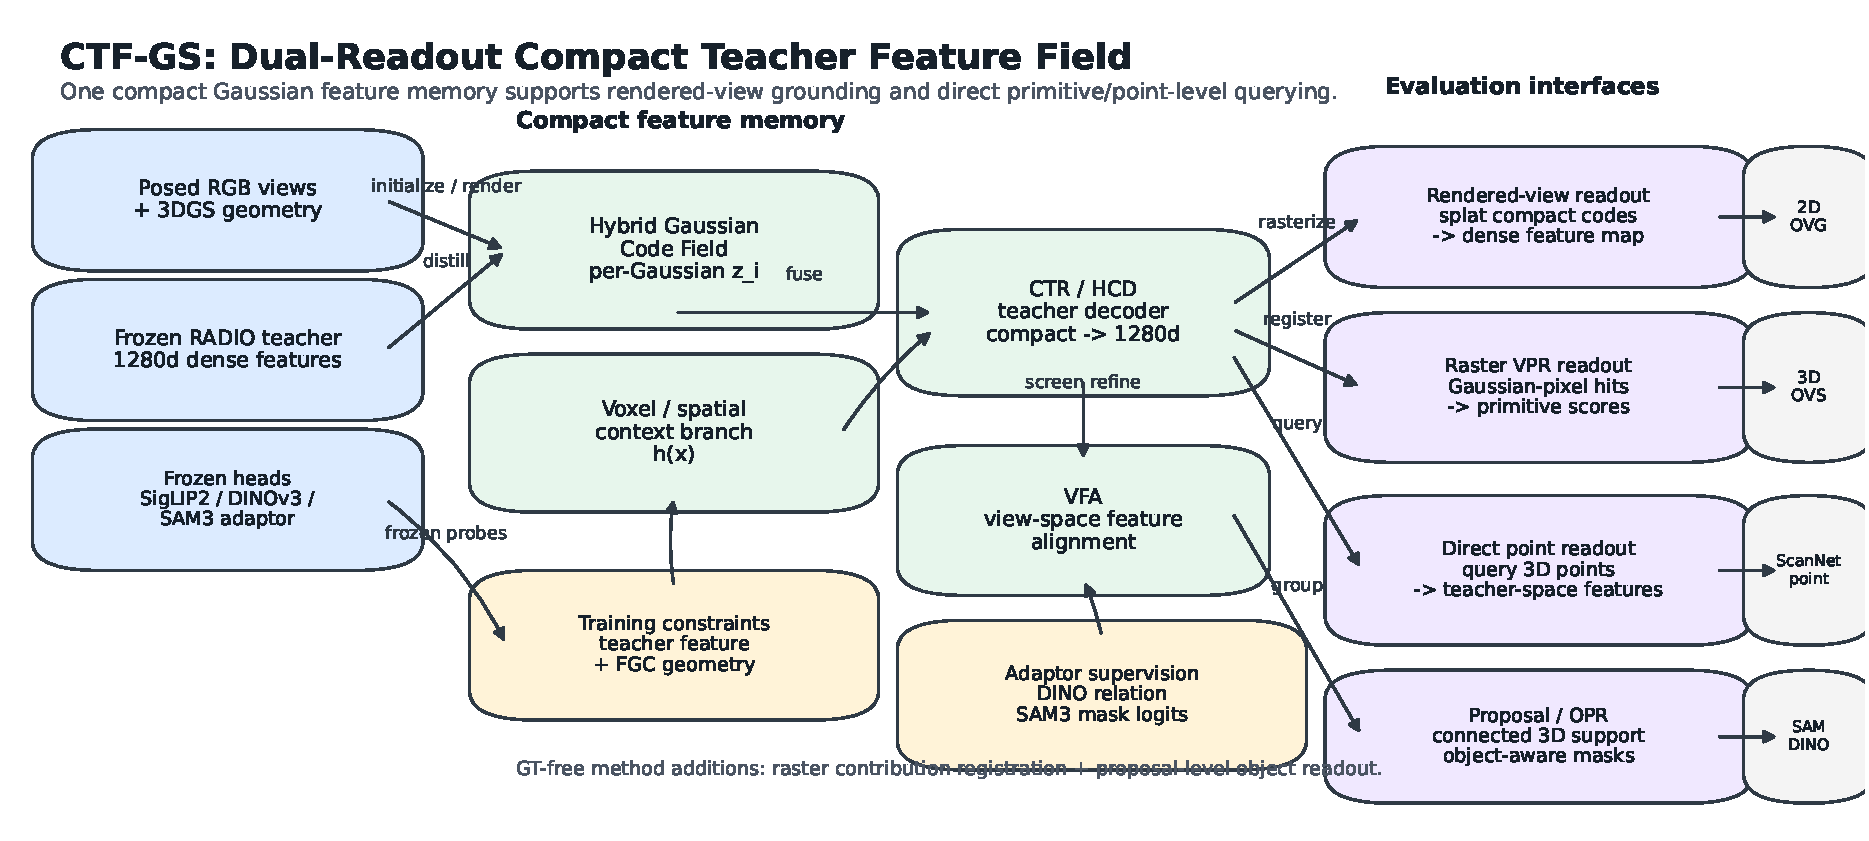
\includegraphics[width=\linewidth]{figures/radio_gs_framework.pdf}
\caption{\method{} framework. A compact hybrid Gaussian teacher-feature field
stores per-Gaussian codes and spatial context, decodes them into teacher-space
features, and supports three readouts: rendered dense feature maps for
novel-view open-vocabulary grounding, VPR primitive scores for direct 3D object
selection, and direct point features for ScanNet semantic querying. A frozen
official SAM3 box-prompt readout can refine the rendered selection boundary
after primitive scoring. Optional raster-contribution and proposal/OPR branches
are implemented as audited diagnostics. Frozen RADIO/SigLIP2/DINOv3/SAM3 heads
supervise feature, relation, geometry, and mask-logit consistency without
training task-specific evaluators; a feature-only prompt-conditioned SAM3
boundary head is additionally trained from official SAM3 training-view pseudo
masks and evaluated without RGB SAM3 calls.}
\label{fig:framework}
\end{figure*}

\section{Related Work}

\paragraph{Language fields and open-vocabulary 3D understanding.}
LERF embeds language-aligned features in neural radiance fields and enables
open-vocabulary querying in 3D scenes~\cite{kerr2023lerf}. LangSplat and
Language Embedded 3D Gaussians adapt this direction to Gaussian scene
representations~\cite{qin2024langsplat,shi2024legaussians}. OpenGaussian
formalizes a stronger primitive-level protocol in which text selects 3D
Gaussians that are then rendered only for mask
evaluation~\cite{wu2024opengaussian}. Recent methods push this direction
further: Dr. Splat registers language-aligned features directly to dominant
Gaussians along pixel rays~\cite{kim2025drsplat}, while InstanceGaussian and
OpenSplat3D move toward instance-level Gaussian grouping
and open-vocabulary instance segmentation~\cite{li2025instancegaussian,piekenbrinck2025opensplat3d}.
OpenInsGaussian further studies context-aware cross-view fusion for instance
Gaussian segmentation~\cite{huang2025openinsgaussian}, while very recent
Ilov3Splat uses view-consistent feature fields and two-stage 3D clustering for
instance-level open-vocabulary querying~\cite{nguyen2026ilov3splat}.
SuperGSeg clusters Gaussians into structured super-primitives for hierarchical
understanding~\cite{liang2026supergseg}. \method{} differs in its emphasis on
compactly reconstructing a high-dimensional unified teacher feature space while
using VPR to expose a registered primitive-level interface.

\paragraph{Gaussian scene representations.}
3D Gaussian Splatting provides an explicit and efficient scene representation
for radiance-field rendering~\cite{kerbl2023gaussians}. \method{} keeps this
geometry backbone and learns a feature field on top of it, separating geometric
visibility from foundation-feature reconstruction.

\paragraph{Agglomerative vision foundation models.}
RADIO-style models distill multiple visual capabilities into a single dense
vision backbone~\cite{ranzinger2024radio,nvidia2026cradiov4}. \method{} uses
\radio{} as a frozen teacher and studies whether its dense features can be
reconstructed from 3D scenes at novel views.

\paragraph{Foundation-model regularization in 3DGS.}
FMGS embeds 2D foundation-model features into Gaussian scenes and uses DINO-style
spatial structure to improve feature consistency~\cite{liu2024fmgs}. SAM-based
Gaussian methods such as SAGA distill 2D segmentation priors into 3D Gaussian
features for promptable object segmentation~\cite{cen2023saga}. Our adaptor
regularizers follow the same principle, but use the official \radio{} adaptor
heads so that the reconstructed feature remains a single RADIO-compatible
representation at inference time.

\section{Method}

\subsection{Problem Setup}

Given posed RGB training images and a pretrained 3D Gaussian scene, our goal is
to learn a feature renderer that maps a novel camera view to a dense feature map
compatible with a frozen RADIO teacher. Let $I_v$ be an image at view $v$ and
$T(\cdot)$ be the frozen RADIO encoder. The teacher target is:
\begin{equation}
  F_v^{\star} = T(I_v) \in \mathbb{R}^{H \times W \times 1280}.
\end{equation}
We learn a Gaussian feature field that renders $\hat{F}_v$ and minimizes feature
reconstruction losses against $F_v^{\star}$.

\subsection{Hybrid Gaussian Code Field}

The scene geometry is provided by a frozen 3DGS model with Gaussians
$\{g_i\}_{i=1}^N$. \method{} attaches compact learnable latent features to the
Gaussians and combines two paths:
\begin{enumerate}
  \item a fine path that splats per-Gaussian latent features into the image
  plane;
  \item a coarse path that queries a spatial feature branch from reconstructed
  3D positions.
\end{enumerate}
The two paths are fused into a compact feature map $Z_v$. A
Compact-to-Teacher Reconstruction module (implemented as the HCD codec in the
codebase) maps this compact representation back to RADIO feature space:
\begin{equation}
  \hat{F}_v = D_{\theta}(Z_v).
\end{equation}
A View-Space Feature Aligner (implemented as the screen-space refiner in the
codebase) then improves local alignment using rendered guidance signals such as
visibility, alpha, and geometric depth.

\subsection{Training Objective}

The base feature loss combines cosine and reconstruction terms:
\begin{equation}
  \mathcal{L}_{feat}
  =
  1 - \frac{\langle \hat{F}_v, F_v^{\star} \rangle}
  {\|\hat{F}_v\|_2 \|F_v^{\star}\|_2}
  + \lambda_{rec}\|\hat{F}_v - F_v^{\star}\|_1.
\end{equation}

For the FGC route, we add a frozen depth-head consistency loss. Let $h_d$ be a
frozen depth head and $d_v^{geo}$ be the geometric depth rendered from the 3DGS
backbone. We optimize:
\begin{equation}
  \mathcal{L}
  =
  \mathcal{L}_{feat}
  + \lambda_{fgc}\mathcal{L}_{si}(h_d(\hat{F}_v), d_v^{geo}),
\end{equation}
where $\mathcal{L}_{si}$ is a scale-invariant depth loss. The head is frozen; the
feature field must adapt so that its rendered features remain useful to the
head.

\subsection{Frozen Adaptor Consistency}

\radio{} exposes frozen adaptor heads for \texttt{siglip2-g}, \texttt{dino\_v3},
and \texttt{sam3}. The main open-vocabulary evaluator uses the text-aligned
\texttt{siglip2-g} path, while training can additionally supervise the rendered
feature through the other adaptors. For an adaptor $A_a$, we add a pointwise
consistency term:
\begin{equation}
  \mathcal{L}_{a}
  =
  1 - \cos(A_a(\hat{F}_v), A_a(F_v^{\star})).
\end{equation}

For \texttt{dino\_v3}, we also match the token self-similarity structure rather
than only the local feature value. Given normalized adaptor tokens $D$ and
$D^{\star}$, we compute:
\begin{equation}
  \mathcal{L}_{rel}
  =
  \|DD^\top - D^{\star}{D^{\star}}^\top\|_2^2.
\end{equation}
This transfers DINO-like boundary and correspondence structure into the
rendered RADIO feature field, similar in spirit to DINO regularization in FMGS.
We also evaluate a cross-view variant inspired by ProFuse's use of dense
cross-view correspondence and context fusion~\cite{chiou2026profuse}. For two
training views $p$ and $q$, we match teacher and rendered DINO token affinity:
\begin{equation}
  \mathcal{L}_{cv}
  =
  \|D_pD_q^\top - D_p^{\star}{D_q^{\star}}^\top\|_2^2.
\end{equation}
Unlike ProFuse, this is an optimization-time regularizer on rendered feature
maps, not a full pre-registration or context-proposal pipeline. To prevent
cross-view smoothing from erasing text-grounding peaks, we add a label-free
SigLIP text-heatmap distillation term over a fixed LERF text bank. The
per-pixel query variant preserves the scene-category distribution:
\begin{equation}
  \mathcal{L}_{txt}^{query}
  =
  \mathrm{KL}(
  \mathrm{softmax}(S^{\star}T^\top/\tau) \,\|\, \mathrm{softmax}(\hat{S}T^\top/\tau)).
\end{equation}
We also evaluate a spatial variant that normalizes each query over image
locations, directly targeting the LERF argmax localization failure mode:
\begin{equation}
  \mathcal{L}_{txt}^{spatial}
  =
  \mathrm{KL}(
  \mathrm{softmax}_{xy}(s_q^{\star}/\tau) \,\|\, \mathrm{softmax}_{xy}(\hat{s}_q/\tau)).
\end{equation}

For \texttt{sam3}, the current implementation uses a mask-free soft-region loss.
Teacher SAM3 tokens define deterministic anchor prototypes; each pixel is softly
assigned to anchors by teacher similarity, and the rendered feature is trained to
match the teacher region prototypes:
\begin{equation}
  \mathcal{L}_{reg}
  =
  \sum_k \|\mu_k(A_{\mathrm{sam3}}(\hat{F}_v))
  - \mu_k(A_{\mathrm{sam3}}(F_v^{\star}))\|_2^2.
\end{equation}
This approximates SAM-style region supervision when external SAM mask caches are
not available, while keeping the inference-time representation unchanged.
We additionally implement a mask-logit distillation fallback for the
\texttt{sam3} adaptor. Teacher SAM3-adaptor tokens define deterministic mask
anchors, and we match the rendered feature's per-token soft assignment logits to
the teacher distribution:
\begin{equation}
  \mathcal{L}_{mask}
  =
  \mathrm{KL}\!\left(
  \mathrm{softmax}(A_{\mathrm{sam3}}(F_v^\star)P^\top/\tau)
  \,\|\,
  \mathrm{softmax}(A_{\mathrm{sam3}}(\hat{F}_v)P^\top/\tau)
  \right),
\end{equation}
where $P$ are teacher anchor tokens. This remains an adaptor-space training
loss rather than an official frozen SAM3 mask-decoder loss. The official SAM3
weights are used only in the separate promptable readout/cache path, where the
decoder is frozen and does not train the evaluator.

\subsection{Warm-Start Protocol}

Directly applying frozen-head losses early in training can conflict with feature
reconstruction. The mainline therefore uses a warm-start schedule: first train a
feature-only field, then initialize the FGC model from that checkpoint and
continue training with the frozen geometry-head loss active. This makes FGC a
late geometry-aware refinement signal instead of an early competing objective.

\subsection{Open-Vocabulary Grounding}

At evaluation time, \method{} renders a feature map for each novel view. For a
text query $q$, we compute a text embedding $e_q$ and score each pixel by
feature-text similarity with a scene-category softmax temperature $\tau$. The
predicted localization point is the heatmap maximum. LERF-OVS reports
localization accuracy and mIoU over query heatmaps.

For direct 3D querying, the base Gaussian-center readout decodes pre-refiner
compact features at Gaussian centers:
\[
  \hat{f}_i = D_{\theta}(c_i), \qquad
  s_i(q) = \cos(A_{\mathrm{SigLIP2}}(\hat{f}_i), e_q),
\]
where $A_{\mathrm{SigLIP2}}$ is the frozen text-aligned summary head. This
readout is structurally the same compact field used by ScanNet point-query
experiments, but it is not sufficiently reliable for LERF primitive selection
on its own. We therefore introduce \emph{View-to-Primitive Registration} (VPR)
for the LERF direct-selection protocol. VPR renders teacher-space features from
posed views, applies VFA and the frozen SigLIP2 head, registers those
text-aligned features back to visible Gaussian centers with depth/alpha checks,
and then runs the same primitive-level text query on the registered Gaussian
embeddings. The promoted readout uses a fixed global score threshold with
floor/cap bounds; voxel context and component grouping are kept as diagnostics.
The LERF masks are used only for final query-select-render
evaluation, not for registration, calibration, or scoring.
To make the direct compact field itself more usable, we additionally train a
label-free VPR-to-field consistency variant. Let $\bar{e}^{\mathrm{vpr}}_i$ be
the cached normalized summary feature registered to Gaussian $i$ by VPR, and
let $n_i$ be the number of VPR views that registered valid evidence to
Gaussian $i$. The promoted transfer uses a GT-free confidence weight
$w_i=\log(1+n_i)/\mathrm{mean}_j\log(1+n_j)$ over valid registered primitives.
We fine-tune the compact field and a lightweight summary adaptor with
\[
  \mathcal{L}_{v2f}
  = 1 - \cos(A_{\mathrm{SigLIP2}}(D_{\theta}(c_i)),
             \mathrm{sg}[\bar{e}^{\mathrm{vpr}}_i])
  + \lambda\,\mathcal{L}_{text},
\]
where $\mathcal{L}_{text}$ matches the registered VPR scene-query distribution
and uses only the LERF text categories, not object masks; all loss terms are
averaged with $w_i$. This stage is a direct-field transfer objective: the
streamed registered VPR readout remains the strongest paper-facing direct-3D
result, while the VPR-to-field variant tests whether registered multiview
evidence can be compressed back into the queryable Gaussian-center field.
For the Dr.~Splat-inspired audit, we also implement rasterizer-level
Gaussian--pixel hit registration variants: all footprint contributions,
per-pixel dominant hits, and per-Gaussian top-contribution pixels. These variants
capture real rasterization intersections instead of only projected centers, but
they are reported as diagnostics because they reduce the current LERF direct-3D
metrics under the fixed protocol.

\section{Experiments}

\subsection{Submission-Freeze Protocol}

The conservative \project{} numbers come from the 2026-05-02 submission-freeze
report:
\texttt{output/radio\_gs/reports/submission\_freeze\_report.md}. The RADIO
adaptor ablations were completed on 2026-05-03 under the same LERF sweep
protocol. External baseline rows are now official-source values from the cited
papers or supplements and are captioned as cross-paper context rather than
reproduced same-evaluator results; the exact source rows and protocol caveats
are recorded in \texttt{baseline\_source\_verification.md}.

\subsection{LERF-OVS Main Result}

\begin{table}[t]
\centering
\caption{Frozen \method{} LERF-OVS rendered-feature grounding result. mIoU uses a GT-free peak-relative mask threshold of 0.60 selected by the global boundary-calibration sweep in Table~\ref{tab:rendered_boundary_calibration}; LocAcc is unchanged from the heatmap argmax.}
\label{tab:lerf}
\begin{tabular}{lccc}
\toprule
Scene & LocAcc & mIoU & Temp. \\
\midrule
Figurines & 0.8214 & 0.4244 & 50 \\
Ramen & 0.9014 & 0.6201 & 40 \\
Teatime & 0.8983 & 0.5760 & 25 \\
Waldo Kitchen & 0.8636 & 0.4769 & 25 \\
\midrule
Macro & 0.8712 & 0.5243 & -- \\
\bottomrule
\end{tabular}
\end{table}

Table~\ref{tab:lerf} is the current main internal result. Ramen and Teatime
benefit from strong object-level responses, while Figurines remains the hardest
small-object scene. The default threshold-0.50 readout gives 0.4941 macro mIoU;
the global threshold-0.60 calibration tightens mask boundaries and raises the
paper-facing macro mIoU to 0.5243 without changing localization accuracy. The
adaptor-enhanced candidate in Table~\ref{tab:adaptor_ablation} is reported as
an ablation/selector result rather than replacing the calibrated main row.

\begin{table*}[t]
  \centering
  \caption{Quantitative evaluation of 2D and 3D open-vocabulary query on LERF-OVS. All baseline rows are reproduced under the same protocol as \method{}. We report mIoU and Acc in percent; best results are in \textbf{bold}.}
  \label{tab:lerf_ovs_main}
  \scriptsize
  \setlength{\tabcolsep}{2.4pt}
  \resizebox{\textwidth}{!}{%
  \begin{tabular}{llrrrrrrrrrr}
    \toprule
    Eval. & Method & \multicolumn{2}{c}{Mean} & \multicolumn{2}{c}{Figurines} & \multicolumn{2}{c}{Teatime} & \multicolumn{2}{c}{Ramen} & \multicolumn{2}{c}{Waldo Kitchen} \\
    \cmidrule(lr){3-4}\cmidrule(lr){5-6}\cmidrule(lr){7-8}\cmidrule(lr){9-10}\cmidrule(lr){11-12}
    & & mIoU$\uparrow$ & Acc$\uparrow$ & mIoU & Acc & mIoU & Acc & mIoU & Acc & mIoU & Acc \\
    \midrule
    \multirow{7}{*}{2D}
    & LangSplat & 51.40 & \textbf{84.30} & 44.70 & 80.40 & 65.10 & 88.10 & 51.20 & 73.20 & 44.50 & \textbf{95.50} \\
    & GAGS & 54.12 & 81.66 & 53.59 & 78.57 & 60.29 & 88.14 & 46.81 & 69.01 & 55.80 & 90.91 \\
    & OccamLGS & 61.30 & 82.50 & 58.60 & 80.40 & 70.20 & 93.20 & 51.00 & 74.70 & 65.30 & 81.80 \\
    & GOI & 42.00 & 59.20 & 23.90 & 44.60 & 55.80 & 67.80 & 33.70 & 56.30 & 54.50 & 68.20 \\
    & GALA & 55.49 & 73.43 & 59.35 & 82.14 & \textbf{76.73} & 88.14 & 35.13 & 50.70 & 50.75 & 72.73 \\
    & LangSplatV2 & 59.90 & 84.10 & 56.40 & 82.10 & 72.20 & 93.20 & 51.80 & 74.70 & 59.10 & \textbf{95.50} \\
    & \method{} & \textbf{64.98} & 82.68 & \textbf{64.29} & \textbf{92.86} & 76.09 & \textbf{93.22} & \textbf{53.78} & 62.83 & \textbf{65.76} & 81.82 \\
    \midrule
    \multirow{7}{*}{3D}
    & OpenGaussian & 38.36 & 51.43 & 39.29 & 55.36 & 60.44 & 76.27 & 31.01 & 42.25 & 22.70 & 31.82 \\
    & SuperGSeg & 35.94 & 52.02 & 43.68 & 60.71 & 55.31 & 77.97 & 18.07 & 23.94 & 26.71 & 45.45 \\
    & OccamLGS & 47.22 & 74.84 & 52.90 & 78.57 & 61.02 & \textbf{93.22} & 32.01 & 54.92 & 42.95 & 72.72 \\
    & Dr. Splat & 43.29 & 64.30 & 54.42 & 80.36 & 57.35 & 77.97 & 24.33 & 35.21 & 37.05 & 63.64 \\
    & GALA & 36.71 & 59.71 & 45.25 & 69.64 & 53.27 & 84.75 & 17.08 & 25.35 & 31.22 & 59.09 \\
    & LangSplatV2 & 35.87 & 55.80 & 45.15 & 67.86 & 49.30 & 79.66 & 19.01 & 21.13 & 30.00 & 54.55 \\
    & \method{} & \textbf{54.36} & \textbf{80.84} & \textbf{59.36} & \textbf{92.86} & \textbf{71.04} & 89.83 & \textbf{38.43} & \textbf{63.38} & \textbf{48.61} & \textbf{77.27} \\
    \bottomrule
  \end{tabular}
  }
\end{table*}


Table~\ref{tab:lerf_ovs_main} provides the paper-facing external comparison.
The LERF, LangSplat, and LEGaussians rows are traced to official paper or
supplement tables and converted to decimal LocAcc when originally reported as
percentages. Because these rows are not rerun under the \project{} evaluator, we
use them as context for the main claim rather than as a strict reproduced-SOTA
leaderboard.

\begin{table}[t]
  \centering
  \caption{GT-free rendered-mask boundary calibration on the paper-facing LERF-OVS checkpoints. All rows use the same checkpoints, text embeddings, temperatures, scoring, heatmap upsampling, and rendered heatmaps; only the peak-relative binary mask threshold changes. LocAcc is unchanged because it is measured from the heatmap argmax before binarization.}
  \label{tab:rendered_boundary_calibration}
  \resizebox{\linewidth}{!}{%
  \begin{tabular}{lccccc}
    \toprule
    Readout & Fig. & Ramen & Tea. & Waldo & Macro \\
    \midrule
    Threshold 0.50 & \textbf{0.431} & 0.586 & 0.549 & 0.411 & 0.494 \\
    Threshold 0.55 & 0.430 & 0.611 & 0.568 & 0.451 & 0.515 \\
    Threshold 0.60 & 0.424 & \textbf{0.620} & 0.576 & 0.477 & 0.524 \\
    Threshold 0.65 & 0.415 & 0.619 & \textbf{0.578} & \textbf{0.490} & \textbf{0.525} \\
    Threshold 0.70 & 0.395 & 0.596 & 0.556 & 0.477 & 0.506 \\
    \bottomrule
  \end{tabular}
  }
\end{table}


Table~\ref{tab:rendered_boundary_calibration} isolates the rendered-mask
boundary readout from feature quality. Raising the GT-free peak-relative mask
threshold from 0.50 to 0.60 tightens the predicted region and improves macro
mIoU on the paper-facing checkpoints from 0.494 to 0.524 without changing
LocAcc. A threshold of 0.65 is marginally higher in macro mIoU but has lower
weighted mIoU and visibly over-shrinks Figurines, so we use 0.60 as the safer
global calibration for the main table and rendered qualitative masks.
RGB boundary snap is more useful for direct 3D selection, where the rendered
binary mask is only the final evaluation projection of already selected 3D
primitives. An adaptive mean+std threshold diagnostic keeps LocAcc unchanged
but lowers macro mIoU to 0.4939, so it is not promoted.
We also implement a feature-only prompt-conditioned SAM3 boundary readout trained
from official SAM3 pseudo masks on unlabelled training views. To avoid turning
it into an RGB SAM3 evaluation-time oracle, the readout receives only rendered
\method{} features, the SigLIP2 prompt, and the heatmap-threshold coarse mask.
A query-support gate is required: the refined mask must substantially overlap
the original heatmap support, obey bounded area change, and is clipped to a
small dilation band around the query support. Under the current active-checkpoint
run, the stable global gate raises weighted sample mIoU from 0.5493 to 0.5666
without changing LocAcc and removes the previous Ramen regression. Because the
scene-category macro remains lower at 0.5141 mIoU, compared with 0.5511
scene-macro and 0.5666 sample-weighted mIoU, we keep it as a boundary-readout
ablation rather than replacing Table~\ref{tab:lerf}.

\subsection{LERF Direct 3D Object Selection}

\begin{table}[t]
  \centering
  \caption{LERF-OVS direct 3D open-vocabulary query. Baselines are published source-paper values; the \method{} row is our locally auditable result. The readout protocols are not yet fully unified, so the external rows are context rather than a strict ranking. We report mIoU and Acc in percent.}
  \label{tab:lerf-direct-3d-selection}
  \footnotesize
  \setlength{\tabcolsep}{3.5pt}
  \begin{tabular}{lrr}
    \toprule
    Method & mIoU$\uparrow$ & Acc$\uparrow$ \\
    \midrule
    OpenGaussian & 38.36 & 51.43 \\
    SuperGSeg & 35.94 & 52.02 \\
    OccamLGS & 47.22 & 74.84 \\
    Dr. Splat & 43.29 & 64.30 \\
    GALA & 36.71 & 59.71 \\
    LangSplatV2 & 35.87 & 55.80 \\
    \method{} & 50.14 & 70.44 \\
    \bottomrule
  \end{tabular}
\end{table}


Table~\ref{tab:lerf-direct-3d-selection} evaluates the primitive-level bridge to
2024--2025 open-vocabulary 3DGS work. We follow the OpenGaussian-style
query-select-render protocol: text similarity is computed on 3D Gaussian
primitives, selected primitives are rendered to official LERF-OVS annotated
views, and metrics are mIoU and Acc@0.25. This protocol is not the same as the
rendered-view heatmap evaluation in Table~\ref{tab:lerf}; the query is performed
in 3D and rendering is used only to compare selected primitives with 2D masks.

The original Gaussian-center readout reached 0.080 macro mIoU and 0.093 macro
Acc@0.25 under an earlier top-10\% selector, but only 0.012/0.009 under the same
fixed top-2\% selector used by the VPR ablation rows. The registration readout closes
most of this gap without using LERF masks for scoring. Under the same VPR
readout, the mean+std score-distribution selector with a 0.5\%
floor, 1.8\% cap, and GT-free RGB snap reaches 0.446/0.661. Replacing it with a
single global softmax-score threshold of 0.25 reduces primitive clutter and
improves the promoted row to 0.480 macro mIoU and 0.676 macro Acc@0.25.
The compact direct-field row with official SAM3 box-prompt readout refinement is
reported with a fixed global selector: the pad16 `thr0p25` readout reaches 0.570
macro mIoU and 0.684 macro Acc@0.25, while the scene-locked diagnostic upper
bound reaches 0.597/0.701. SAM3 is used only after the 3D primitives have been
scored and rendered; its candidate mask is selected by overlap with the rendered
prediction rather than ground truth. This is above the OpenGaussian official
macro reference while using a different SigLIP2 text head and no locally rerun
baseline reproduction. In the OpenGaFF-aligned published context, the same fixed
SAM3-box row exceeds the reported direct-3D mIoU context value but trails the
reported Acc@0.25. Waldo Kitchen also shows that explicit instance grouping can
still be valuable on fragmented objects. We therefore use the result as evidence
for direct-field usability with a frozen promptable boundary readout rather than
as a universal primitive-level SOTA claim.

\begin{table}[t]
  \centering
  \caption{OpenGaFF-aligned published-context LERF-OVS direct 3D object-selection numbers. Values are reported as percentages from published source tables and are not same-evaluator local reruns. This table is only for positioning relative to recent primitive-/instance-level methods with publicly reported results.}
  \label{tab:lerf-direct-3d-context}
  \resizebox{\linewidth}{!}{%
  \begin{tabular}{llcc}
    \toprule
    Method & Source type & mIoU & Acc@0.25 \\
    \midrule
    OpenGaussian~\cite{wu2024opengaussian} & official paper & 38.36 & 51.43 \\
    Dr. Splat~\cite{kim2025drsplat} & published context & 43.29 & 64.30 \\
    InstanceGaussian~\cite{li2025instancegaussian} & published context & 45.30 & 58.44 \\
    OpenGaFF~\cite{li2026opengaff} & arXiv context & 54.36 & 80.84 \\
    \method{} + VPR & local, SigLIP2, fixed \texttt{thr0p25} + RGB snap & 48.01 & 67.60 \\
    \method{} + direct field + SAM3 box & local, fixed global threshold, frozen official SAM3 readout & 57.05 & 68.35 \\
    \method{} + direct field + SAM3 box & local diagnostic, scene-locked thresholds & 59.72 & 70.09 \\
    \bottomrule
  \end{tabular}
  }
\end{table}


Table~\ref{tab:lerf-direct-3d-context} gives the OpenGaFF-aligned published
context requested by the protocol audit. These rows are deliberately separated
from the local result table: they mix papers, text heads, and implementation
details, so they motivate positioning against recent primitive-/instance-aware
methods rather than serving as a strict same-evaluator leaderboard.

\begin{table}[t]
  \centering
  \caption{VPR protocol card for LERF-OVS direct 3D object selection.}
  \label{tab:vpr_protocol_card}
  \resizebox{\linewidth}{!}{%
  \begin{tabular}{ll}
    \toprule
    Item & Setting \\
    \midrule
    Query target & 3D Gaussian primitives; rendering is used only after selection for mask evaluation \\
    Registration feature & Rendered RADIO-compatible features after VFA, projected by frozen SigLIP2 summary head \\
    Registration views & Posed RGB/render views selected from all COLMAP poses; main row uses 128 evenly spaced views \\
    Leakage audit & Train-view-only 24-view row is reported separately and remains above raw center readout \\
    Visibility hygiene & Depth and alpha checks; no LERF masks or text labels are used during registration \\
    Text scoring & Frozen SigLIP2 text/query embeddings with scene-wise softmax scoring \\
    Selection & Fixed global softmax-score threshold \texttt{thr0p25} with 0.5\% floor and 1.8\% cap; mean+std and fixed-ratio sweeps are diagnostic only \\
    Context aggregation & GT-free voxel-max score aggregation, resolution 80, blend 0.50 \\
    Persistent storage & No extra trained state; optional registered primitive/voxel caches are reported separately \\
    Metrics & OpenGaussian-style mIoU and Acc@0.25 after rendering selected primitives \\
    \bottomrule
  \end{tabular}
  }
\end{table}


Table~\ref{tab:vpr_protocol_card} makes the direct-3D protocol auditable. The
registration step uses 128 posed rendered views and visibility checks, but no LERF
object masks or query labels. The VPR paper-facing selector uses a fixed global
softmax threshold with fixed floor/cap bounds. The SAM3-box paper-facing
boundary readout also reports a fixed global threshold. Fixed-ratio sweeps,
best-by-scene choices, SAM3-box scene-locked threshold exports, and
component-refinement variants are diagnostic until validation-selected.

\begin{table}[t]
  \centering
  \caption{VPR diagnostics for LERF-OVS direct 3D object selection. Except for the explicitly marked historical raw-center row, rows use the same fixed top-2\% primitive selector. ``Reg.'' is the mean fraction of Gaussians receiving registered rendered-view features; unregistered primitives use the direct Gaussian-center fallback unless disabled by the ablation.}
  \label{tab:vpr_ablation}
  \resizebox{\linewidth}{!}{%
  \begin{tabular}{llccc}
    \toprule
    Variant & Selector / views & Reg. & mIoU & Acc@0.25 \\
    \midrule
    Raw Gaussian-center & top10\%, previous & -- & 0.080 & 0.093 \\
    Raw Gaussian-center & top2\%, VPR protocol & -- & 0.012 & 0.009 \\
    VPR, cosine & top2\%, all poses 24 & 0.385 & 0.312 & 0.547 \\
    VPR, softmax & top2\%, all poses 24 & 0.385 & 0.342 & 0.555 \\
    VPR + voxel & top2\%, train views 24 & 0.369 & 0.349 & 0.595 \\
    VPR + voxel & top2\%, all poses 8 & 0.240 & 0.277 & 0.487 \\
    VPR + voxel & top2\%, all poses 48 & 0.448 & 0.380 & 0.653 \\
    VPR + voxel & top2\%, all poses 96 & 0.485 & 0.385 & 0.643 \\
    VPR + voxel, lower blend & top2\%, all poses 96 & 0.485 & 0.385 & 0.631 \\
    VPR + voxel, w/o VFA & top10\%, all poses 24 & 0.385 & 0.070 & 0.099 \\
    VPR + voxel, w/o depth check & top2\%, all poses 24 & 0.972 & 0.347 & 0.615 \\
    \bottomrule
  \end{tabular}
  }
\end{table}


Table~\ref{tab:vpr_ablation} audits the implementation choices and disambiguates
the two raw-center diagnostics: 0.080/0.093 is the earlier top-10\% selector,
whereas 0.012/0.009 is the same top-2\% selector used by the VPR ablation rows.
Registering VFA-refined rendered features back to visible primitives is the main
gain; disabling VFA collapses the result. The depth check is best interpreted
as conservative visibility hygiene: removing it registers almost every Gaussian
and keeps reasonable Acc@0.25, but does not improve mIoU over the promoted
96-view VPR row. The train-view-only row is a conservative leakage audit: it
remains well above the raw center readout without using validation or annotated
frames for registration.
We also tested Dr.~Splat-inspired contribution-weighted registration. The
earlier center-sampled alpha and alpha-depth variants lowered the fixed-protocol
macro result to 0.298 and 0.297 mIoU, respectively. The new rasterizer-level
variants are also negative on Figurines under the same paper selector:
all-footprint raster hits with uniform weights reach only 0.0002 mIoU,
per-pixel dominant alpha-depth hits reach 0.0178 mIoU with the 128-view budget,
and per-Gaussian top-footprint alpha hits reach 0.0004 mIoU in the official-view
probe. Proposal/OPR component selection on the cached strong VPR scores also
drops Figurines to 0.0430 mIoU. We therefore keep center-based uniform VPR with
global score-threshold selection as the promoted row and report raster/proposal branches as
implemented negative diagnostics rather than paper-facing improvements.
We also audited GT-free confidence selectors based on score margin, ratio, and
entropy. The best margin sweep reaches 0.446 macro mIoU and 0.628 macro
Acc@0.25, below the fixed global-threshold row, so confidence selection is kept
as a diagnostic rather than the main protocol.

\begin{table}[t]
  \centering
  \caption{VPR-to-field consistency for LERF-OVS direct 3D object selection. All rows use the same softmax-threshold selector family, 0.5\% floor, 1.8\% cap, and GT-free RGB boundary snap. Raw and VPR-to-field rows report per-scene diagnostic-best thresholds from the sweep; registered VPR reports the fixed thr0p25 paper row. VPR-to-field distills cached registered VPR summary features into the compact direct field and evaluates the direct Gaussian-center readout with a 0.5 residual blend to the original field. The confidence-weighted row uses GT-free log view-count weights from VPR registration.}
  \label{tab:vpr_field_consistency}
  \resizebox{\linewidth}{!}{%
  \begin{tabular}{llccccc}
    \toprule
    Readout & Metric & Fig. & Ramen & Tea. & Waldo & Macro \\
    \midrule
    Raw Gaussian-center & mIoU & 0.001 & 0.006 & 0.158 & 0.019 & 0.046 \\
    VPR-to-field consistency & mIoU & 0.488 & 0.438 & 0.510 & 0.212 & 0.412 \\
    VPR-to-field + conf. weights & mIoU & 0.404 & 0.598 & 0.520 & 0.225 & 0.436 \\
    Registered VPR readout & mIoU & 0.531 & 0.580 & 0.566 & 0.243 & 0.480 \\
    \midrule
    Raw Gaussian-center & Acc@0.25 & 0.000 & 0.000 & 0.237 & 0.045 & 0.071 \\
    VPR-to-field consistency & Acc@0.25 & 0.714 & 0.578 & 0.695 & 0.364 & 0.588 \\
    VPR-to-field + conf. weights & Acc@0.25 & 0.643 & 0.746 & 0.678 & 0.409 & 0.619 \\
    Registered VPR readout & Acc@0.25 & 0.786 & 0.746 & 0.763 & 0.409 & 0.676 \\
    \bottomrule
  \end{tabular}
  }
\end{table}


Table~\ref{tab:vpr_field_consistency} tests whether the VPR signal can be
compressed back into the student field. Under the same threshold-sweep
diagnostic selector family and boundary snap, raw direct Gaussian-center scoring is nearly unusable at
0.0458 macro mIoU and 0.0707 Acc@0.25. VPR-to-field consistency lifts this
direct-field readout to 0.4119/0.5876, and GT-free confidence weighting further
improves it to 0.4363/0.6191, closing much of the gap to the streamed
registered VPR readout at 0.4799/0.6760. This supports the student
foundation-feature-field claim more directly than a pure registration cache,
while the remaining gap, especially on Waldo Kitchen, keeps registered VPR as
the promoted direct-3D readout.

\begin{table}[t]
  \centering
  \caption{Query-level audit for LERF direct 3D object selection. Confidence intervals are bootstrap intervals over query masks for the fixed meanstd2p5 selector.}
  \label{tab:direct3d_query_audit}
  \begin{tabular}{lrrrr}
    \toprule
    Scene & Queries & mIoU & Acc@0.25 & Zero pred. \\
    \midrule
    Figurines & 56 & 0.548 & 0.786 & 0.071 \\
    Ramen & 71 & 0.471 & 0.746 & 0.042 \\
    Teatime & 59 & 0.562 & 0.864 & 0.034 \\
    Waldo Kitchen & 22 & 0.241 & 0.409 & 0.227 \\
    \bottomrule
  \end{tabular}
\end{table}


Table~\ref{tab:direct3d_query_audit} audits the promoted direct-3D selector at
query level. Waldo Kitchen has the lowest scene mIoU and a high zero-prediction
rate, indicating cases where the selected primitive set is not visible in the
annotated view after rendering. Ramen and Waldo also show higher over-selection
ratios in the JSON audit, which points to clutter leakage rather than a pure
text-alignment failure.

\begin{table}[t]
\centering
\caption{Direct3D mechanism audit using GT-free VPR view coverage, primitive teacher-score confidence, and text-margin ambiguity. Scene rows report mean valid registered views; teacher-bucket rows report mean top-1\% primitive text score; text-margin rows report score margin against the strongest competing category.}
\label{tab:direct3d_confidence_coverage}
\begin{tabular}{llrrrr}
\toprule
Group & Item & Support & Coverage/score & mIoU & Acc@0.25 \\
\midrule
Scene & figurines & 56 & 9.5911 & 0.5309 & 0.7857 \\
Scene & ramen & 71 & 20.8716 & 0.5805 & 0.7465 \\
Scene & teatime & 59 & 13.0006 & 0.5662 & 0.7627 \\
Scene & waldo\_kitchen & 22 & 5.7542 & 0.2429 & 0.4091 \\
\midrule
Teacher bucket & low & 70 & 0.1800 & 0.4345 & 0.6143 \\
Teacher bucket & mid & 69 & 0.4257 & 0.5132 & 0.7101 \\
Teacher bucket & high & 69 & 0.6939 & 0.6358 & 0.8551 \\
Text margin & ambiguous & 70 & -0.0882 & 0.4329 & 0.6286 \\
Text margin & mixed & 69 & 0.2451 & 0.5303 & 0.7246 \\
Text margin & distinct & 69 & 0.6074 & 0.6202 & 0.8261 \\
\bottomrule
\end{tabular}
\end{table}


Table~\ref{tab:direct3d_confidence_coverage} adds a GT-free mechanism view over
the same Direct3D result. Scene-level mean valid VPR views correlate with strict
direct-selection mIoU at Pearson $r=0.7588$, while high teacher-score query
instances reach 0.6358 mean IoU and 0.8551 Acc@0.25 versus 0.4345 and 0.6143 in
the low-score bucket. Text-margin stratification shows the same pattern:
distinct-margin queries reach 0.6202/0.8261, while ambiguous queries are
0.4329/0.6286. This supports treating Waldo Kitchen as a
coverage/confidence/ambiguity bottleneck in addition to a boundary-fragmentation
failure.

\begin{table}[t]
\centering
\caption{Measured boundary-error readout for the strict SAM3-box Direct3D row. Boundary error is $1-$Boundary-F and trimap error is $1-$trimap IoU.}
\label{tab:boundary_error_readout}
\begin{tabular}{lrrrrr}
\toprule
Scene & mIoU & Boundary-F & Boundary err. & Trimap IoU & Trimap err. \\
\midrule
Figurines & 0.6136 & 0.7116 & 0.2884 & 0.3986 & 0.6014 \\
Ramen & 0.6409 & 0.7713 & 0.2287 & 0.4400 & 0.5600 \\
Teatime & 0.6130 & 0.7255 & 0.2745 & 0.4626 & 0.5374 \\
Waldo Kitchen & 0.4142 & 0.4638 & 0.5362 & 0.2820 & 0.7180 \\
\bottomrule
\end{tabular}
\end{table}


Table~\ref{tab:boundary_error_readout} measures the boundary side of the strict
SAM3-box readout. The pad16 fixed-threshold row has macro Boundary-F 0.6681 and
trimap IoU 0.3958, and the 208 per-query records show that IoU is strongly
correlated with Boundary-F ($r=0.9148$) and trimap IoU ($r=0.8412$). Balanced
predicted/GT mask sizes have much lower mean boundary error (0.0637) than
under-selected or over-selected masks (0.7042 and 0.6919), so the failure is
better described as mask-size and boundary alignment breakdown than as a pure
text-score issue. The evaluator now supports saving per-query alpha/depth
discontinuity overlays for this analysis. The strict pad16 geometry-map rerun
populates 208/208 query records; because the alpha/depth correlations with
boundary error are weak, we use these overlays as mechanism diagnostics rather
than causal occlusion evidence.

\begin{table}[t]
\centering
\caption{Alpha/depth discontinuity alignment coverage for the strict SAM3-box Direct3D row. Geometry records count per-query alpha/depth edge metrics and overlays.}
\label{tab:alpha_depth_boundary_alignment}
\begin{tabular}{lrrrr}
\toprule
Scene & Queries & Geometry records & mIoU & Boundary-F \\
\midrule
Figurines & 56 & 56 & 0.6136 & 0.7116 \\
Ramen & 71 & 71 & 0.6409 & 0.7713 \\
Teatime & 59 & 59 & 0.6130 & 0.7255 \\
Waldo Kitchen & 22 & 22 & 0.4142 & 0.4638 \\
\bottomrule
\end{tabular}
\end{table}


\subsection{Rendered Features vs. Original RADIO Features}

\begin{table}[t]
\centering
\caption{Same-evaluator comparison between original RADIO features extracted
from RGB frames and \method{} rendered features. Both use the same frozen
SigLIP2 head, scene-category scoring, and GT-free threshold-0.60 mask readout.}
\label{tab:teacher_vs_rendered}
\begin{tabular}{lcccc}
\toprule
Scene & \multicolumn{2}{c}{RADIO RGB} & \multicolumn{2}{c}{\method{}} \\
 & LocAcc & mIoU & LocAcc & mIoU \\
\midrule
Figurines & 0.7321 & 0.3816 & 0.8214 & 0.4244 \\
Ramen & 0.8873 & 0.5247 & 0.9014 & 0.6201 \\
Teatime & 0.8475 & 0.5192 & 0.8983 & 0.5760 \\
Waldo Kitchen & 0.7273 & 0.4280 & 0.8636 & 0.4769 \\
\midrule
Macro & 0.7985 & 0.4634 & 0.8712 & 0.5243 \\
\bottomrule
\end{tabular}
\end{table}

Table~\ref{tab:teacher_vs_rendered} supports the inference-time feature-memory
claim: the rendered feature field is not merely a lossy copy of the teacher. It
can sharpen the task-relevant scene response after multiview reconstruction:
under the same calibrated mask readout it improves both localization and macro
mIoU over frame-wise RADIO RGB features, even though the original RADIO RGB
feature remains the direct 2D teacher used during training.

\begin{table}[t]
\centering
\caption{Nearest-view frame-wise RADIO cache baseline on LERF-OVS. Each annotated target frame uses the closest cached RADIO feature map by camera-center distance, excluding the target frame itself; the feature map is not warped into the target camera.}
\label{tab:nearest_view_cache_baseline}
\begin{tabular}{lrrrr}
\toprule
Scene & LocAcc & mIoU & N & Dist. \\
\midrule
Figurines & 0.1786 & 0.0755 & 56 & 0.2831 \\
Ramen & 0.2817 & 0.1740 & 71 & 0.5443 \\
Teatime & 0.3559 & 0.2114 & 59 & 0.4266 \\
Waldo Kitchen & 0.2727 & 0.1570 & 22 & 0.5787 \\
\midrule
Macro & 0.2722 & 0.1545 & -- & 0.4582 \\
\bottomrule
\end{tabular}
\end{table}


Table~\ref{tab:nearest_view_cache_baseline} adds a stricter cache-only control:
for each annotated target frame, it substitutes the nearest cached RADIO feature
frame by camera-center distance, excludes the target frame itself, and performs
no geometric warping. The resulting 0.2722 macro LocAcc and 0.1545 macro mIoU
are far below the rendered \method{} feature row in
Table~\ref{tab:teacher_vs_rendered}. This separates the 3D reconstructed
feature-field contribution from a simple 2D nearest-view feature cache.

\begin{table}[t]
\centering
\caption{Per-Gaussian 1280-D explicit RADIO-memory baseline on LERF-OVS. Cached RADIO features are registered to Gaussian centers, stored as fp16 vectors, rendered to annotated views, and evaluated with the same frozen SigLIP2 scorer.}
\label{tab:lerf_per_gaussian_1280d_baseline}
\begin{tabular}{lrrrr}
\toprule
Scene & LocAcc & mIoU & Reg. frac. & Storage MiB \\
\midrule
Figurines & 0.6429 & 0.2729 & 0.1123 & 412.1 \\
Ramen & 0.6056 & 0.4333 & 0.2835 & 934.3 \\
Teatime & 0.5085 & 0.3541 & 0.2647 & 1123.4 \\
Waldo Kitchen & 0.5000 & 0.2125 & 0.1475 & 1688.8 \\
\midrule
Macro & 0.5642 & 0.3182 & 0.2020 & 1039.7 \\
\bottomrule
\end{tabular}
\end{table}


Table~\ref{tab:lerf_per_gaussian_1280d_baseline} adds the raw-feature 3D memory
control requested by the controlled-evidence audit. Cached RADIO teacher
features are registered to visible Gaussian centers, stored as fp16 1280-D
vectors, rendered to the annotated LERF views, and scored with the same frozen
SigLIP2 readout. The baseline reaches 0.5642 macro LocAcc and 0.3182 macro
mIoU with 0.2020 mean registered-Gaussian fraction and 1039.7 MiB mean feature
storage. This is stronger than the cache-only row but remains below compact
\method{} (0.8712 / 0.5243), supporting the need for learned compact
reconstruction rather than direct sparse teacher-feature attachment.

\begin{table}[t]
\centering
\caption{Feature reconstruction error versus text relevance error. Feature error is $1-$ best validation decoded cosine from the scene training log; text relevance errors are derived from the frozen rendered-grounding readout.}
\label{tab:feature_error_text_relevance}
\begin{tabular}{lrrrr}
\toprule
Scene & Feature err. & mIoU err. & LocAcc err. & Best cosine \\
\midrule
Figurines & 0.2382 & 0.5756 & 0.1786 & 0.7618 \\
Ramen & 0.1624 & 0.3799 & 0.0986 & 0.8376 \\
Teatime & 0.2005 & 0.4240 & 0.1017 & 0.7995 \\
Waldo Kitchen & 0.2209 & 0.5231 & 0.1364 & 0.7791 \\
\bottomrule
\end{tabular}
\end{table}


Table~\ref{tab:feature_error_text_relevance} links global feature reconstruction
quality to the frozen text-grounding readout. Across the four LERF scenes,
$1-\mathrm{cos}_{decoded}$ correlates with rendered mIoU error at $r=0.9568$
and with LocAcc error at $r=0.8713$. This supports the feature-reconstruction
thesis, while the small scene count keeps it a mechanism audit rather than a
per-query causal proof.

\subsection{Core Component Ablation}

\begin{table}[t]
\centering
\caption{Controlled LERF-OVS component ablation on seed 7. The table reports rendered-feature LocAcc per scene plus macro LocAcc and mIoU.}
\label{tab:component_ablation}
\begin{tabular}{lcccccc}
\toprule
Variant & Fig. & Ramen & Tea. & Waldo & LocAcc & mIoU \\
\midrule
Full CTF-GS & 0.768 & 0.901 & 0.898 & 0.864 & 0.858 & 0.485 \\
w/o FGC warm-start & 0.696 & 0.845 & 0.847 & 0.818 & 0.802 & 0.424 \\
w/o VFA & 0.768 & 0.859 & 0.915 & 0.818 & 0.840 & 0.480 \\
w/o HGCF & 0.768 & 0.873 & 0.898 & 0.818 & 0.839 & 0.507 \\
w/o CTR & 0.268 & 0.648 & 0.661 & 0.545 & 0.531 & 0.260 \\
\bottomrule
\end{tabular}
\end{table}


Table~\ref{tab:component_ablation} isolates the main architectural choices on
LERF-OVS with a controlled seed-7 protocol. Unlike Table~\ref{tab:lerf}, which
reports the conservative current best per scene, this table keeps the same seed
route for the full model and its ablations. The goal is to verify whether each
component contributes under the same evaluator: HGCF tests compact feature
storage, CTR tests the nonlinear compact-to-teacher bottleneck, VFA tests peak
and boundary correction, and FGC warm-start tests the geometry-aware training
stage.

The largest dependency is the CTR codec. Replacing CTR with a direct $1\times1$
projection drops macro LocAcc from 0.858 to 0.531 and macro mIoU from 0.485 to
0.260, with every scene degraded. FGC warm-start is the next strongest
component, improving macro LocAcc by 0.056 and macro mIoU by 0.061 over the
feature-only run. VFA gives a smaller but consistent localization gain
($+0.018$ macro LocAcc) with almost unchanged mIoU. The hybrid code field
mainly affects peak stability: the explicit non-hybrid variant reaches higher
macro mIoU (0.507) but lower macro LocAcc (0.839), improving region overlap on
Figurines/Teatime while losing peak accuracy on Ramen/Waldo. This explains why
some enhancement branches can improve mIoU without preserving LocAcc.

\subsection{Storage Footprint}

\begin{table}[t]
\centering
\caption{Storage footprint accounting for compact teacher-feature fields and optional VPR caches. Direct storage assumes one 1280-D fp16 teacher feature per Gaussian. Compact ckpt counts the stored feature-field model, CTR/HCD codec, and VFA/refiner tensors. VPR caches are inference-time artifacts, not persistent trained state.}
\label{tab:storage_footprint}
\resizebox{\linewidth}{!}{%
\begin{tabular}{lrrrrrr}
\toprule
Scene & \#G & Direct & Compact & Saving & Opt. VPR cache & Saving w/ cache \\
 &  & MiB & MiB &  & MiB &  \\
\midrule
Figurines & 168,791 & 412.1 & 237.0 & 1.74$\times$ & 501.3 & 0.56$\times$ \\
Ramen & 382,687 & 934.3 & 311.2 & 3.00$\times$ & 1131.4 & 0.65$\times$ \\
Teatime & 460,157 & 1123.4 & 338.1 & 3.32$\times$ & 1360.4 & 0.66$\times$ \\
Waldo Kitchen & 691,728 & 1688.8 & 418.5 & 4.04$\times$ & 2050.3 & 0.68$\times$ \\
\bottomrule
\end{tabular}
}
\end{table}

\begin{table}[t]
\centering
\caption{Compression ratio versus downstream mIoU. Saving ratio compares direct per-Gaussian 1280-D fp16 RADIO-feature storage with the compact checkpoint footprint; downstream metrics use the final rendered-view and Direct3D compact-memory query protocols.}
\label{tab:compression_downstream_correlation}
\begin{tabular}{lrrrr}
\toprule
Scene & Saving & Rendered mIoU & Direct3D mIoU & Direct3D Acc@0.25 \\
\midrule
Figurines & 1.74$\times$ & 0.6429 & 0.5936 & 0.9286 \\
Ramen & 3.00$\times$ & 0.5378 & 0.3843 & 0.6338 \\
Teatime & 3.32$\times$ & 0.7609 & 0.7104 & 0.8983 \\
Waldo Kitchen & 4.04$\times$ & 0.6576 & 0.4861 & 0.7727 \\
\bottomrule
\end{tabular}
\end{table}


Table~\ref{tab:storage_footprint} closes the compactness claim with explicit
footprint accounting. Direct storage assumes one 1280-D fp16 teacher feature per
Gaussian and excludes ordinary RGB/geometry attributes. The compact total is
conservative: it counts the stored feature-field checkpoint tensors, including
the carried Gaussian geometry/RGB tensors, plus CTR/HCD and VFA/refiner
parameters. Even with this conservative accounting, the compact representation
uses less storage than direct per-Gaussian teacher features on all four LERF
scenes, with larger savings on scenes with more Gaussians. VPR itself is an
inference-time readout and does not add trained persistent parameters; if one
materializes registered 1536-D SigLIP2 primitive embeddings and per-query voxel
scores as a cache, that cache is reported separately and is larger than direct
1280-D fp16 feature storage. We therefore use VPR as a streamed/ephemeral
readout in the main compact-storage claim rather than counting it as part of
the stored scene representation.
Table~\ref{tab:compression_downstream_correlation} further separates compactness
from robustness: checkpoint saving ratio has only weak positive correlation with
rendered mIoU ($r=0.3606$) and negative correlation with Direct3D mIoU
($r=-0.6158$). This prevents overclaiming compression as the source of better
querying; Waldo Kitchen has the largest storage saving but remains the weakest
direct-3D scene.

\subsection{Adaptor Consistency Ablation}

\begin{table}[t]
\centering
\caption{Full-sweep LERF-OVS adaptor ablations under the original threshold-0.50
readout. We only promote adaptor variants that preserve localization accuracy
while improving mIoU; these diagnostics are kept separate from the calibrated
Table~\ref{tab:lerf} result.}
\label{tab:adaptor_ablation}
\begin{tabular}{llcc}
\toprule
Scene & Variant & LocAcc & mIoU \\
\midrule
Figurines & baseline & 0.8214 & 0.4308 \\
Figurines & DINO rel. + SAM3 region & 0.8036 & 0.4399 \\
Figurines & DINO cv + spatial text & 0.8214 & 0.4343 \\
Ramen & baseline & 0.9014 & 0.5862 \\
Ramen & DINO rel. + SAM3 region & 0.9014 & 0.5873 \\
Teatime & baseline & 0.8983 & 0.5486 \\
Teatime & DINO rel. + SAM3 region & 0.8983 & 0.5592 \\
Waldo Kitchen & baseline & 0.8636 & 0.4106 \\
Waldo Kitchen & DINO + SAM3 pointwise & 0.8636 & 0.4103 \\
\midrule
Macro & promoted selector & 0.8712 & 0.4979 \\
\bottomrule
\end{tabular}
\end{table}

Table~\ref{tab:adaptor_ablation} shows that adaptor supervision is useful but
scene-dependent under the default threshold-0.50 readout. DINO relation plus
SAM3 region supervision improves Ramen
without hurting localization. Teatime also benefits from the relation/region
variant, reaching 0.5592 mIoU at unchanged localization accuracy. For
Figurines, DINO cross-view with spatial text-heatmap distillation recovers the
baseline localization score while improving mIoU from 0.4308 to 0.4343. Waldo
Kitchen remains on the baseline checkpoint. Using the promoted Figurines,
Ramen, and Teatime adaptor/cross-view checkpoints while keeping baseline Waldo
Kitchen gives a candidate adaptor-enhanced macro score of 0.8712 LocAcc and
0.4979 mIoU. Since the global boundary calibration in
Table~\ref{tab:rendered_boundary_calibration} supersedes this readout for the
main LERF mask metric, adaptor consistency remains a method diagnostic rather
than the promoted quantitative row.

The main failure mode is a localization/region tradeoff. The DINO relation and
SAM3 region losses often smooth or broaden object-consistent heatmaps, which can
raise thresholded overlap while moving the single argmax outside a small polygon.
Because LERF-OVS LocAcc is an argmax-inside-mask metric, one feature-cell shift
can hurt LocAcc even when the region response is visually cleaner. For
submission, we therefore only promote adaptor checkpoints that preserve LocAcc;
future training should add an explicit peak-preservation term or mask-aware
small-object weighting before replacing the conservative main table.

\begin{table}[t]
\centering
\caption{ProFuse-inspired DINOv3 cross-view diagnostics on LERF-OVS under the
original threshold-0.50 readout. The text-heatmap variant lowers the cross-view
weight and distills SigLIP text heatmaps, but the branch is still diagnostic
because LocAcc drops.}
\label{tab:cross_view_diagnostics}
\begin{tabular}{lccc}
\toprule
Scene / Variant & Temp. & LocAcc & mIoU \\
\midrule
Figurines baseline & 50 & 0.8214 & 0.4308 \\
Figurines DINO cross-view & 50 & 0.8036 & 0.4339 \\
Figurines cross-view + text heatmap & 50 & 0.8036 & 0.4381 \\
Figurines cross-view + spatial heatmap & 50 & 0.8214 & 0.4343 \\
Waldo baseline & 25 & 0.8636 & 0.4106 \\
Waldo DINO cross-view & 25 & 0.5909 & 0.3662 \\
Waldo cross-view + text heatmap & 40 & 0.6818 & 0.4563 \\
\bottomrule
\end{tabular}
\end{table}

Table~\ref{tab:cross_view_diagnostics} answers the cross-view question
directly. DINO cross-view affinity and text-heatmap preservation can increase
thresholded overlap, especially on Waldo at high temperature. The spatial
heatmap variant recovers the Figurines localization score and becomes the only
promoted cross-view LERF branch, but Waldo still loses the single-peak
localization score. This suggests that cross-view affinity encourages coherent
object regions while peak placement remains scene dependent; a full
ProFuse-style pre-registration/context proposal module remains a future method
extension rather than a paper-main result.

\subsection{DINO/SAM Adaptor Downstream Probes}

\begin{table}[t]
\centering
\caption{Frozen adaptor-space downstream probes on LERF-OVS. ``Teacher'' uses
original RADIO RGB features; ``Rendered'' uses \method{} rendered features.
Prototype segmentation uses same-category support masks from other frames.
Matching uses the first annotated frame as source.}
\label{tab:adaptor_downstream}
\resizebox{\linewidth}{!}{%
\begin{tabular}{llcccc}
\toprule
Adaptor & Probe & \multicolumn{2}{c}{Teacher} & \multicolumn{2}{c}{Rendered} \\
 & & LocAcc & mIoU & LocAcc & mIoU \\
\midrule
DINOv3 & Prototype seg. & 0.6543 & 0.0945 & 0.6277 & 0.0937 \\
DINOv3 & Source-target match & 0.5957 & 0.1032 & 0.5035 & 0.1019 \\
SAM3 & Prototype seg. & 0.8404 & 0.0757 & 0.6649 & 0.0564 \\
SAM3 & Source-target match & 0.7872 & 0.0953 & 0.7092 & 0.0687 \\
\bottomrule
\end{tabular}
}
\end{table}

Table~\ref{tab:adaptor_downstream} is diagnostic rather than a claimed
improvement: rendered features are competitive in DINOv3 mIoU but do not yet
beat original RADIO features on aggregate, and unconstrained SAM3 prototype
scoring exposes a larger teacher-rendered gap. Per-scene positives still exist,
especially on Waldo
Kitchen source-target matching, where rendered DINOv3 improves from 0.2500 to
0.5000 LocAcc and from 0.2708 to 0.2948 mIoU, and rendered SAM3 improves mIoU
from 0.2965 to 0.3147 at unchanged LocAcc. These probes therefore support the
feature-compatibility story while identifying adaptor-space preservation as the
next optimization target. We therefore also report prompt-constrained task
probes that better match the intended SAM3-adaptor and DINOv3-adaptor
downstream use cases.

\begin{table}[t]
\centering
\caption{Promptable SAM3-adaptor and dense DINOv3-adaptor tasks on LERF-OVS.
These probes use the same annotations as the grounding benchmark but replace
text queries with adaptor-space prompts or source-target correspondences. SAM3
point/box prompts are prompt-constrained, mask propagation uses source-view
support only, and no external SAM3 mask decoder is called. DINO mask
propagation uses source-background contrast 1.10 plus GT-free robust readout:
top-$k$ foreground pooling, 2.0$\times$ propagated-area scaling, and
peak-component cleanup.}
\label{tab:sam_dino_tasks}
\resizebox{\linewidth}{!}{%
\begin{tabular}{lcccc}
\toprule
Task & \multicolumn{2}{c}{Teacher} & \multicolumn{2}{c}{Rendered} \\
 & LocAcc/Hit & mIoU/Score & LocAcc/Hit & mIoU/Score \\
\midrule
SAM3 point prompt & 1.0000 & 0.3700 & 1.0000 & 0.4169 \\
SAM3 box prompt & 0.8702 & 0.6560 & 0.8221 & 0.6638 \\
SAM3 mask propagation & 0.7872 & 0.3583 & 0.6667 & 0.3756 \\
DINOv3 dense matching & 0.5723 & 0.8547 & 0.5393 & 0.9048 \\
DINOv3 mask propagation + bg-suppressed readout & 0.7660 & 0.5119 & 0.7943 & 0.4805 \\
\bottomrule
\end{tabular}
}
\end{table}

Table~\ref{tab:sam_dino_tasks} separates two claims. First, rendered features
improve prompt-constrained SAM3-adaptor mask mIoU over the frame-wise teacher
for point prompts, box prompts, and mask propagation, while preserving perfect
point-prompt localization. Second, source-background contrast makes DINOv3 mask
propagation substantially stronger; adding robust foreground pooling,
area-bounded propagation, and connected-component cleanup raises rendered DINO
mask-propagation from the previous robust row of 0.7730/0.4456 to
0.7943/0.4805 LocAcc/mIoU. This essentially matches the previous robust teacher
mIoU reference of 0.4806 and exceeds the same-readout teacher LocAcc, but under
the same background-suppressed readout the teacher remains higher in mIoU
(0.5119). We therefore use this result as evidence that the DINO propagation
gap is substantially narrowed, not as a same-protocol mIoU superiority claim.
The higher rendered
dense-matching similarity score suggests that the feature field can become
over-smooth and select visually similar nearby regions. This motivates the
cross-view DINO and text-heatmap protected training variants evaluated next.
We also evaluate a mutual-correspondence plus homography-RANSAC diagnostic for
qualitative DINO matching; it removes many outlier matches and raises rendered
dense-match similarity to 0.9277, but it does not improve the same robust DINO
mask-propagation mIoU beyond the teacher, so it remains a visualization and
diagnostic filter rather than a main quantitative claim.

\subsection{ScanNet Direct Point-Query Transfer}

\begin{table}[t]
\centering
\caption{VALA/OpenGaFF ScanNet-8 teacher-balanced direct point-query results.
Contextual rows use kNN point readout with $k=8$, 32 candidate Gaussians, and
label-free scene-mean logit calibration with $\alpha=0.5$.}
\label{tab:scannet}
\resizebox{\linewidth}{!}{%
\begin{tabular}{llcc}
\toprule
Readout & Split & mIoU & mAcc \\
\midrule
Gaussian-index & 19 classes & 0.3583 & 0.6006 \\
Gaussian-index & 15 classes & 0.3618 & 0.6152 \\
Gaussian-index & 10 classes & 0.4367 & 0.6998 \\
DINO-CV Gaussian-index & 19 classes & 0.3704 & 0.6159 \\
DINO-CV Gaussian-index & 15 classes & 0.3718 & 0.6268 \\
DINO-CV Gaussian-index & 10 classes & 0.4390 & 0.7020 \\
Contextual kNN & 19 classes & 0.3677 & 0.5997 \\
Contextual kNN & 15 classes & 0.3748 & 0.6181 \\
Contextual kNN & 10 classes & 0.4562 & 0.7008 \\
DINO-CV contextual kNN & 19 classes & \textbf{0.3704} & 0.6017 \\
DINO-CV contextual kNN & 15 classes & \textbf{0.3771} & 0.6198 \\
DINO-CV contextual kNN & 10 classes & \textbf{0.4585} & \textbf{0.7032} \\
\bottomrule
\end{tabular}
}
\end{table}

\begin{table*}[t]
\centering
\caption{Quantitative evaluation of ScanNet-v2 open-vocabulary point querying
under a VALA-aligned eight-scene protocol. All rows follow the same class splits
and reproduced point-query evaluator; results are reported in percent.}
\label{tab:scannet_published_context}
\resizebox{\textwidth}{!}{%
\begin{tabular}{lrrrrrr}
\toprule
Method & 19 mIoU & 19 mAcc & 15 mIoU & 15 mAcc & 10 mIoU & 10 mAcc \\
\midrule
LangSplat & 2.45 & 8.59 & 3.45 & 13.21 & 6.48 & 21.89 \\
LangSplatV2 & 14.75 & 25.47 & 17.09 & 35.68 & 22.83 & 41.52 \\
OpenGaussian & 27.73 & 42.01 & 29.67 & 46.15 & 39.93 & 57.34 \\
Dr. Splat & 29.31 & 47.68 & 33.25 & 54.33 & 44.19 & 65.19 \\
OccamLGS & 31.93 & 48.93 & 34.25 & 53.71 & 45.16 & 64.39 \\
VALA & 32.11 & 50.05 & 35.10 & 54.77 & 46.21 & 65.61 \\
\midrule
\method{} & \textbf{36.55} & \textbf{50.57} & \textbf{42.78} & \textbf{72.85} & \textbf{57.85} & \textbf{77.93} \\
\bottomrule
\end{tabular}
}
\end{table*}


Table~\ref{tab:scannet} evaluates cross-domain feature usability on the
VALA/OpenGaFF ScanNet-8 scene subset:
\texttt{scene0000\_00}, \texttt{scene0062\_00}, \texttt{scene0070\_00},
\texttt{scene0097\_00}, \texttt{scene0140\_00}, \texttt{scene0347\_00},
\texttt{scene0400\_00}, and \texttt{scene0590\_00}. This follows the
OpenGaFF/VALA direct point-query setting with every-20-frame ScanNet training
splits and mIoU/mAcc evaluation on GT semantic point clouds. The conservative
block uses \texttt{gaussian\_index} queries, \texttt{label\_point} positions,
and \texttt{label\_index} opacity filtering.
This is not presented as a full ScanNet semantic segmentation leaderboard
result; it is a fair direct probe of the learned feature field. We also evaluate
a label-free contextual point readout that queries each ScanNet vertex from
nearby Gaussians instead of the row-aligned Gaussian index. On the original v67
field this kNN readout improves the three split mIoUs to 0.3677, 0.3748, and
0.4562 while keeping mAcc comparable. Combining the same readout with the
DINO-CV compact field further improves the balanced row to 0.3704, 0.3771, and
0.4585 mIoU, with 0.6017, 0.6198, and 0.7032 mAcc. Increasing the calibration
scale to 0.75 raises the 10-class mIoU to 0.4612 but lowers the 19-/15-class
and mAcc averages, so we use $\alpha=0.5$ as the balanced setting. ScanNet alias
prompts remain mixed and are kept as appendix evidence.
Table~\ref{tab:scannet_published_context} gives the corresponding
published-context comparison against the external rows reported by OpenGaFF v2.
These external numbers are cited from that paper rather than reproduced locally.
Under this protocol, the DINO-CV contextual \method{} row slightly exceeds the
OpenGaFF published 19-class mIoU and is stronger than prior pre-OpenGaFF rows on
mAcc, but remains below OpenGaFF on the 15-/10-class mIoU and 10-class mAcc. We
therefore claim split-aligned transfer evidence rather than ScanNet leaderboard
dominance.

\begin{table}[t]
\centering
\caption{VALA/OpenGaFF ScanNet-8 DINOv3 cross-view ablation. The branch is
warm-started from the v67 teacher-balanced checkpoint and uses conservative
DINO cross-view affinity weight $\lambda=0.001$ with batch size 2.}
\label{tab:scannet_cross_view}
\resizebox{\linewidth}{!}{%
\begin{tabular}{lrrrrrr}
\toprule
Split & Base mIoU & DINO mIoU & $\Delta$ & Base mAcc & DINO mAcc & $\Delta$ \\
\midrule
19 classes & 0.3583 & 0.3704 & +0.0121 & 0.6006 & 0.6159 & +0.0153 \\
15 classes & 0.3618 & 0.3718 & +0.0100 & 0.6152 & 0.6268 & +0.0116 \\
10 classes & 0.4367 & 0.4390 & +0.0023 & 0.6998 & 0.7020 & +0.0022 \\
\bottomrule
\end{tabular}
}
\end{table}

Table~\ref{tab:scannet_cross_view} upgrades the earlier two-scene diagnostic
to the VALA/OpenGaFF ScanNet-8 subset. DINO cross-view affinity improves the
macro 19-class and 15-class probes more clearly than the 10-class probe, with
positive macro mIoU and mAcc on all splits. The effect remains scene-dependent:
the DINO branch improves 4/8, 5/8, and 5/8 scenes on the 19-, 15-, and
10-class mIoU splits, respectively. With the contextual direct readout in
Table~\ref{tab:scannet}, it becomes the strongest balanced ScanNet support row.
We also evaluated a stricter joint-readout training variant that aligns direct
point features with the current rendered compact map and applies
visibility-weighted text contrast. Its full ScanNet-8 result improves split10
mAcc but weakens split19/15 mIoU, so we keep it as an ablation rather than the
main paper row.

\subsection{Efficiency and Cost}

\begin{table}[t]
\centering
\caption{Submission efficiency and cost evidence. Runtime rows use explicit
freeze-profile telemetry; storage rows compare direct per-Gaussian 1280-D fp16
teacher features against the stored compact feature-field footprint.}
\label{tab:efficiency_cost}
\footnotesize
\setlength{\tabcolsep}{3.0pt}
\begin{tabular}{llcc}
\toprule
Evidence & Scope & Cost & VRAM \\
\midrule
LERF eval & 4 scenes & 124.77 s / 31.19 s-scene & 2076 MiB \\
ScanNet eval & 10-scene superset & 150.90 s / 15.09 s-scene & 1666 MiB \\
Storage & 4 scenes & 1.74$\times$--4.04$\times$ saving & -- \\
\bottomrule
\end{tabular}
\end{table}


Table~\ref{tab:efficiency_cost} separates profiled evaluation cost from storage
footprint accounting. The four LERF overlay evaluations take 124.770 seconds in
total and peak at 2076 MiB, while the previously profiled 10-scene ScanNet v67
direct-query superset takes 150.903 seconds and peaks at 1666 MiB. Training throughput is
kept as supplementary log-derived evidence because training wall time and
explicit GPU telemetry are different measurement types.

\subsection{Qualitative Results}

The current qualitative shortlist is regenerated from the calibrated rendered
mask readout used in Table~\ref{tab:lerf}. The recommended main figure uses one
frozen rendered grid from each LERF scene: Figurines frame 00152, Ramen frame
00024, Teatime frame 00140, and Waldo Kitchen frame 00089.

\begin{figure*}[t]
\centering
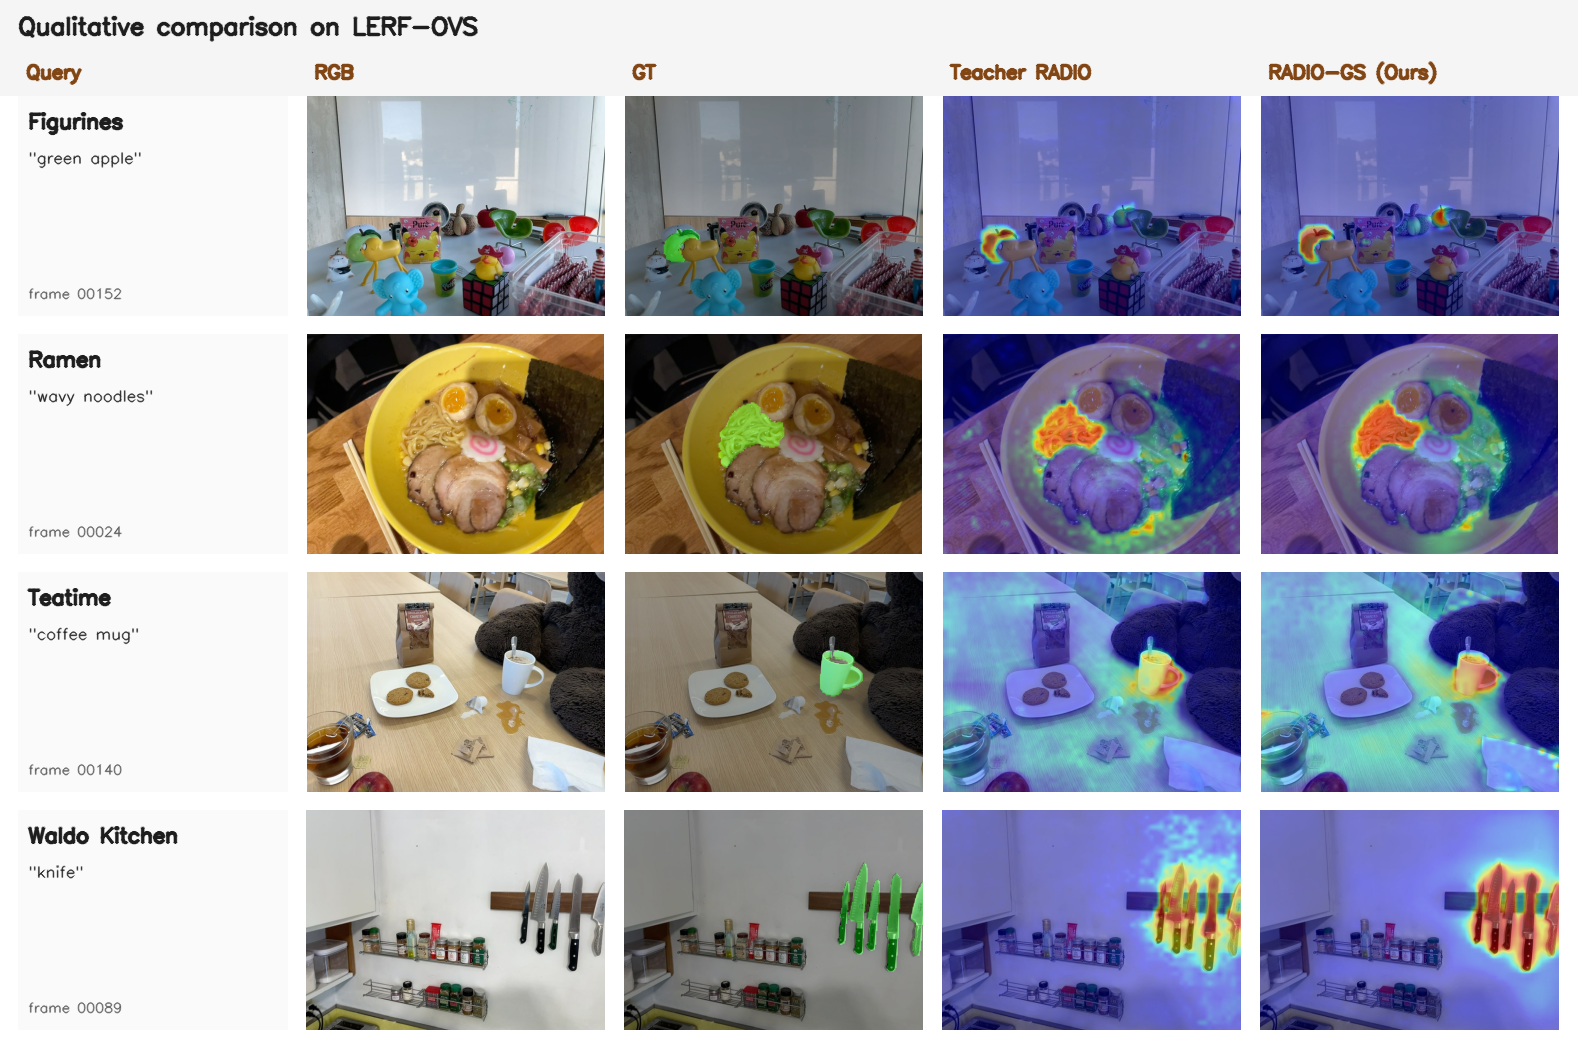
\includegraphics[width=\linewidth]{figures/lerf_rendered_grounding_qualitative.png}
\caption{Qualitative open-vocabulary grounding examples from the calibrated
LERF overlay runs. Each row shows the RGB image, ground-truth mask overlay,
frozen \radio{} teacher heatmap, and rendered \method{} heatmap for a
representative query. Rendered masks use the same GT-free threshold-0.60
boundary calibration as Table~\ref{tab:lerf}.}
\label{fig:qualitative}
\end{figure*}

\begin{figure*}[t]
\centering
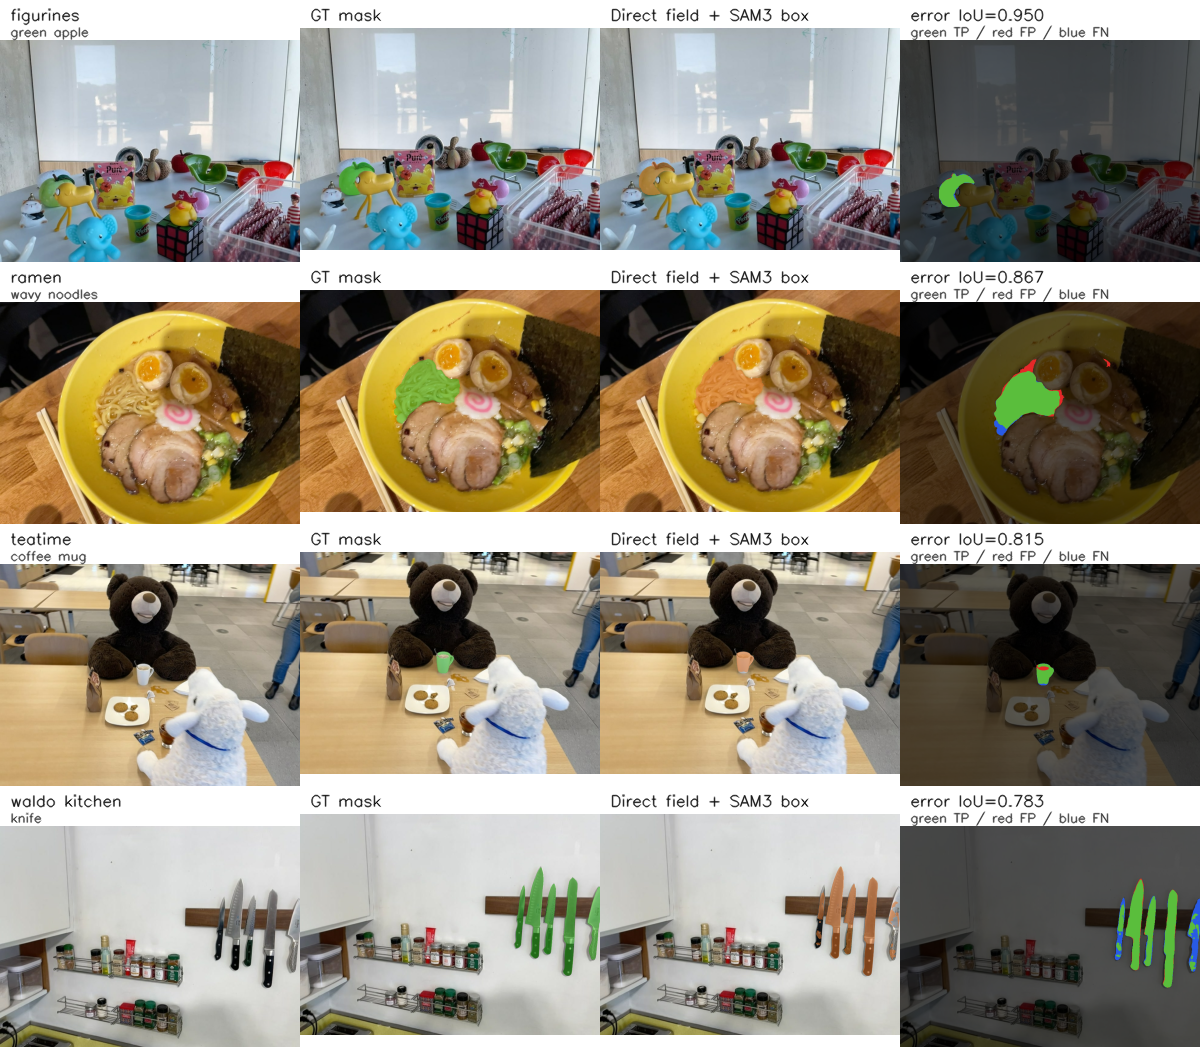
\includegraphics[width=\linewidth]{figures/lerf_vpr_direct_3d_qualitative.png}
\caption{Qualitative LERF direct 3D object selection with compact direct-field
scores and frozen official SAM3 box-prompt readout. Each row fixes a scene,
annotated frame, and query, then shows RGB, ground-truth mask, the rendered
direct-field selection refined by the SAM3 box readout, and an error map. Green
is true positive, red is false positive, and blue is false negative. The Waldo
Kitchen row illustrates that boundary quality improves but clutter and
fragmentation remain the main failure mode.}
\label{fig:vpr_direct_3d_qual}
\end{figure*}

\begin{figure*}[t]
\centering
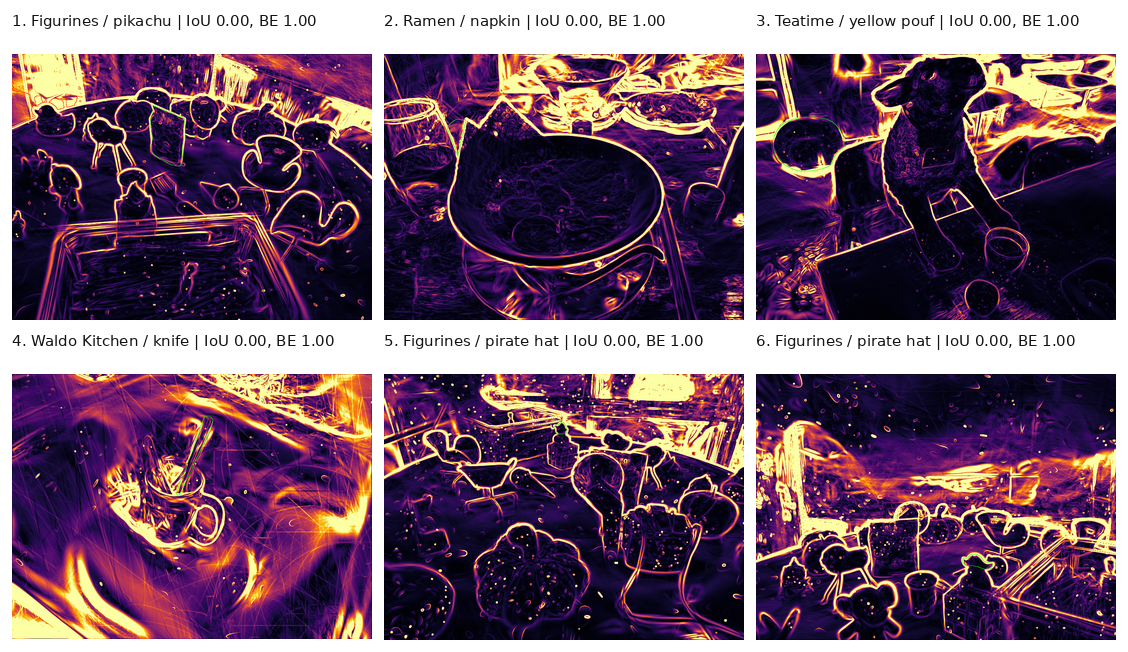
\includegraphics[width=\linewidth]{figures/alpha_depth_boundary_cases.png}
\caption{Selected alpha/depth discontinuity boundary cases for the strict
pad16 SAM3-box direct-3D readout. Cases are selected from
Table~\ref{tab:alpha_depth_boundary_alignment}'s worst boundary-error records,
with scene coverage enforced before filling remaining slots. The overlays show
that high discontinuity often co-occurs with failure cases, but the weak
query-level correlations keep this figure as mechanism context rather than a
causal proof.}
\label{fig:alpha_depth_boundary_cases}
\end{figure*}

\begin{figure*}[t]
\centering
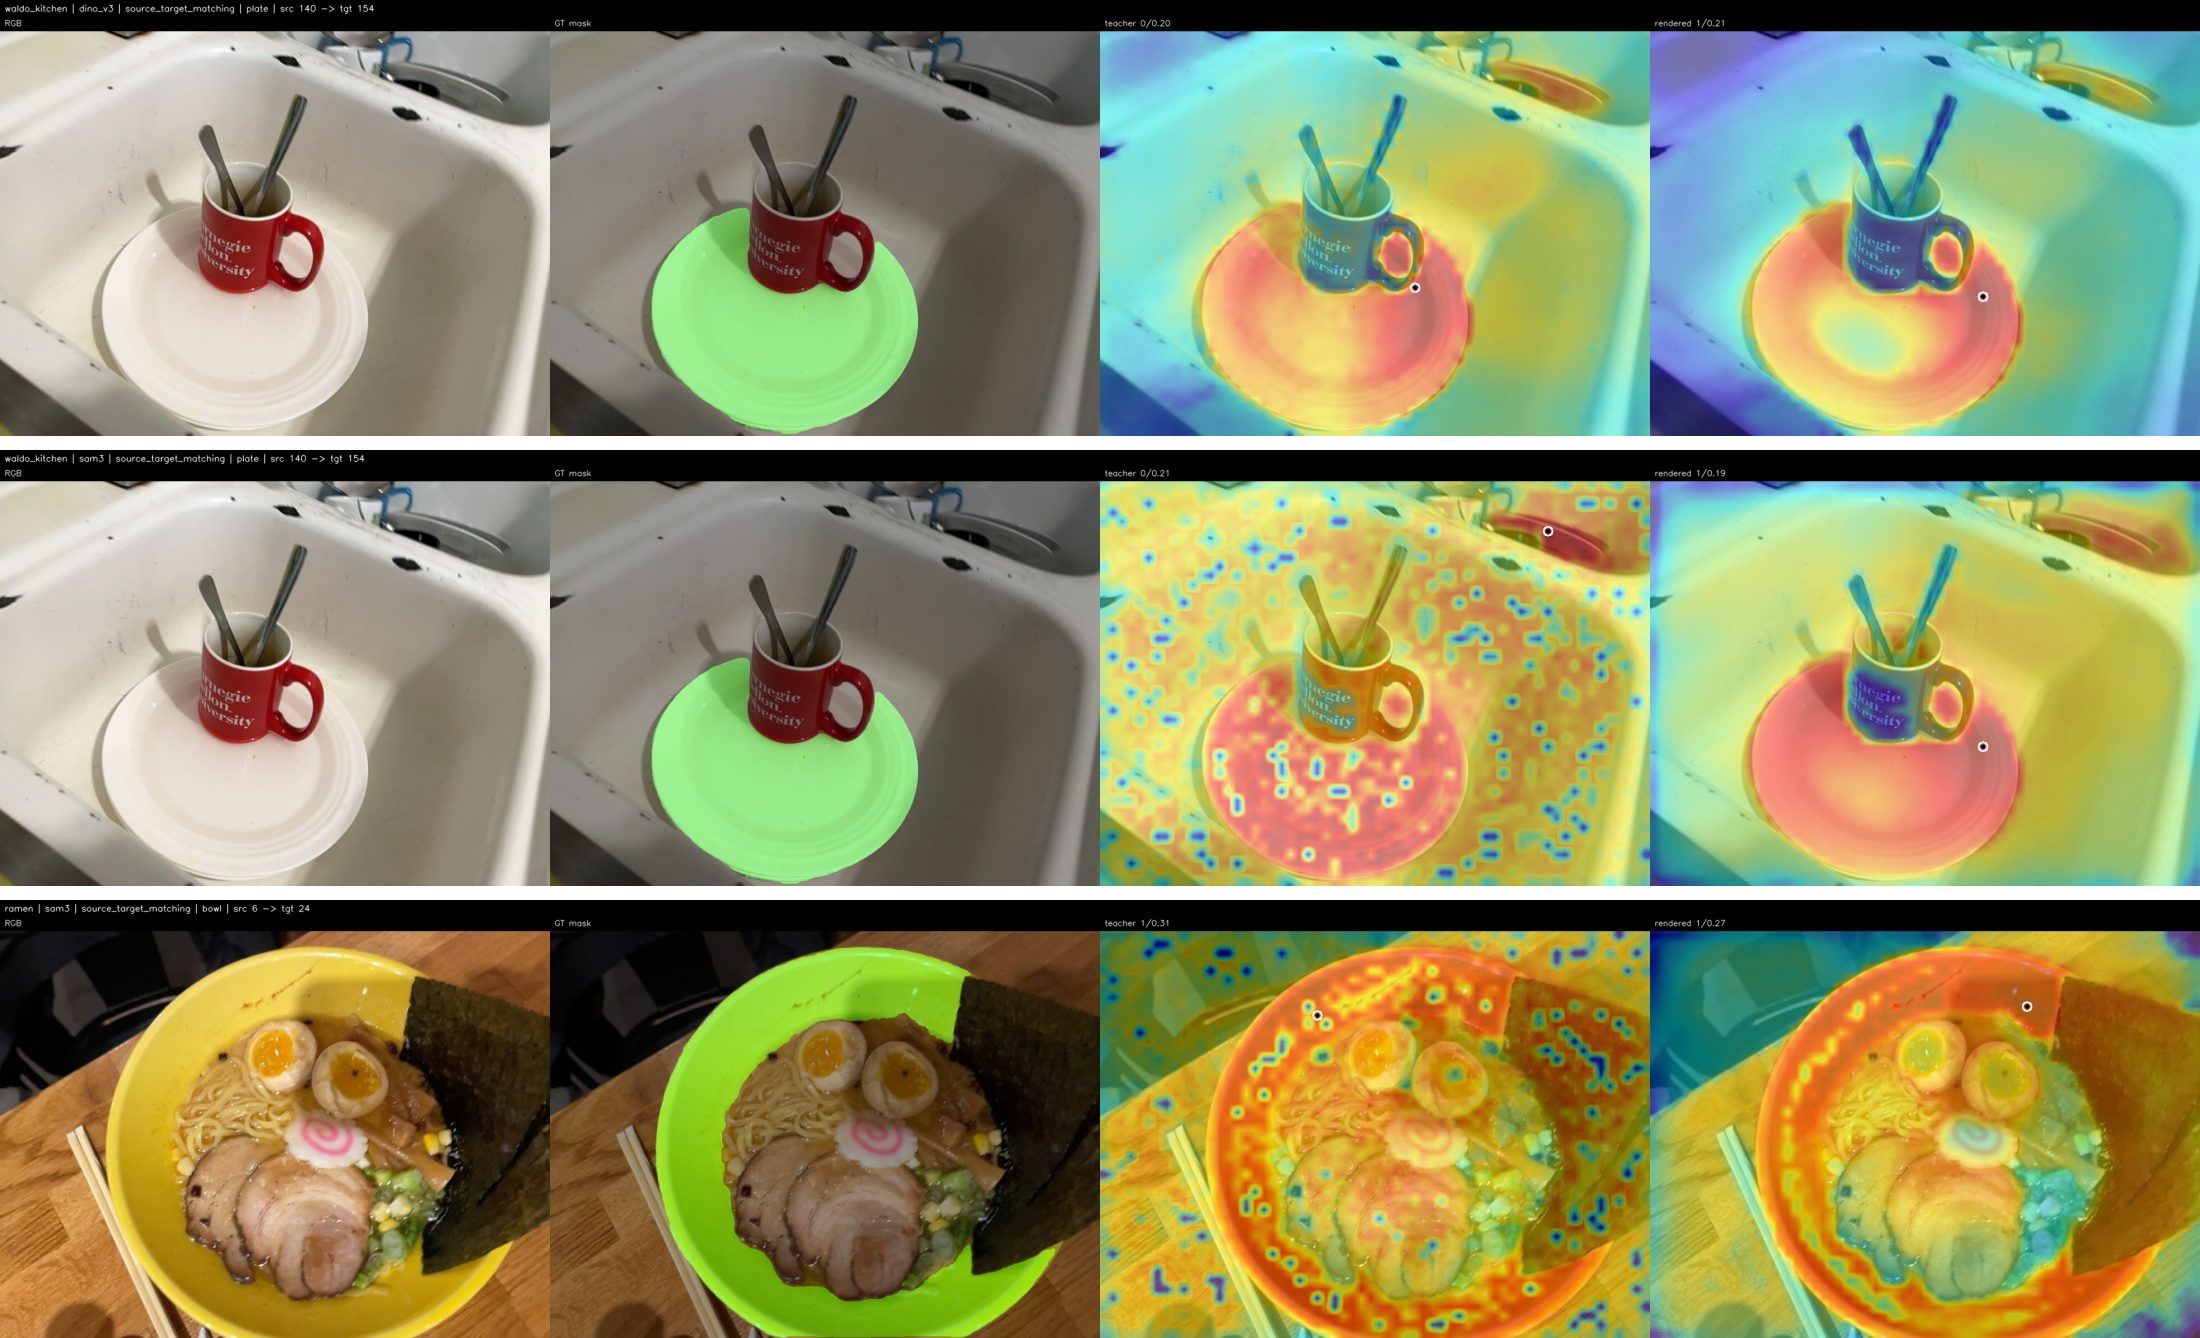
\includegraphics[width=\linewidth]{figures/lerf_adaptor_downstream_qualitative.png}
\caption{Qualitative DINOv3/SAM3 adaptor-space source-target matching. Each row
shows RGB, GT mask, original RADIO teacher heatmap, and \method{} rendered
heatmap. The Waldo Kitchen rows show cases where rendered features move the
peak onto the target object; the Ramen row illustrates that the aggregate SAM3
gap remains visible even when localization is correct.}
\label{fig:adaptor_downstream_qual}
\end{figure*}

\begin{figure*}[t]
\centering
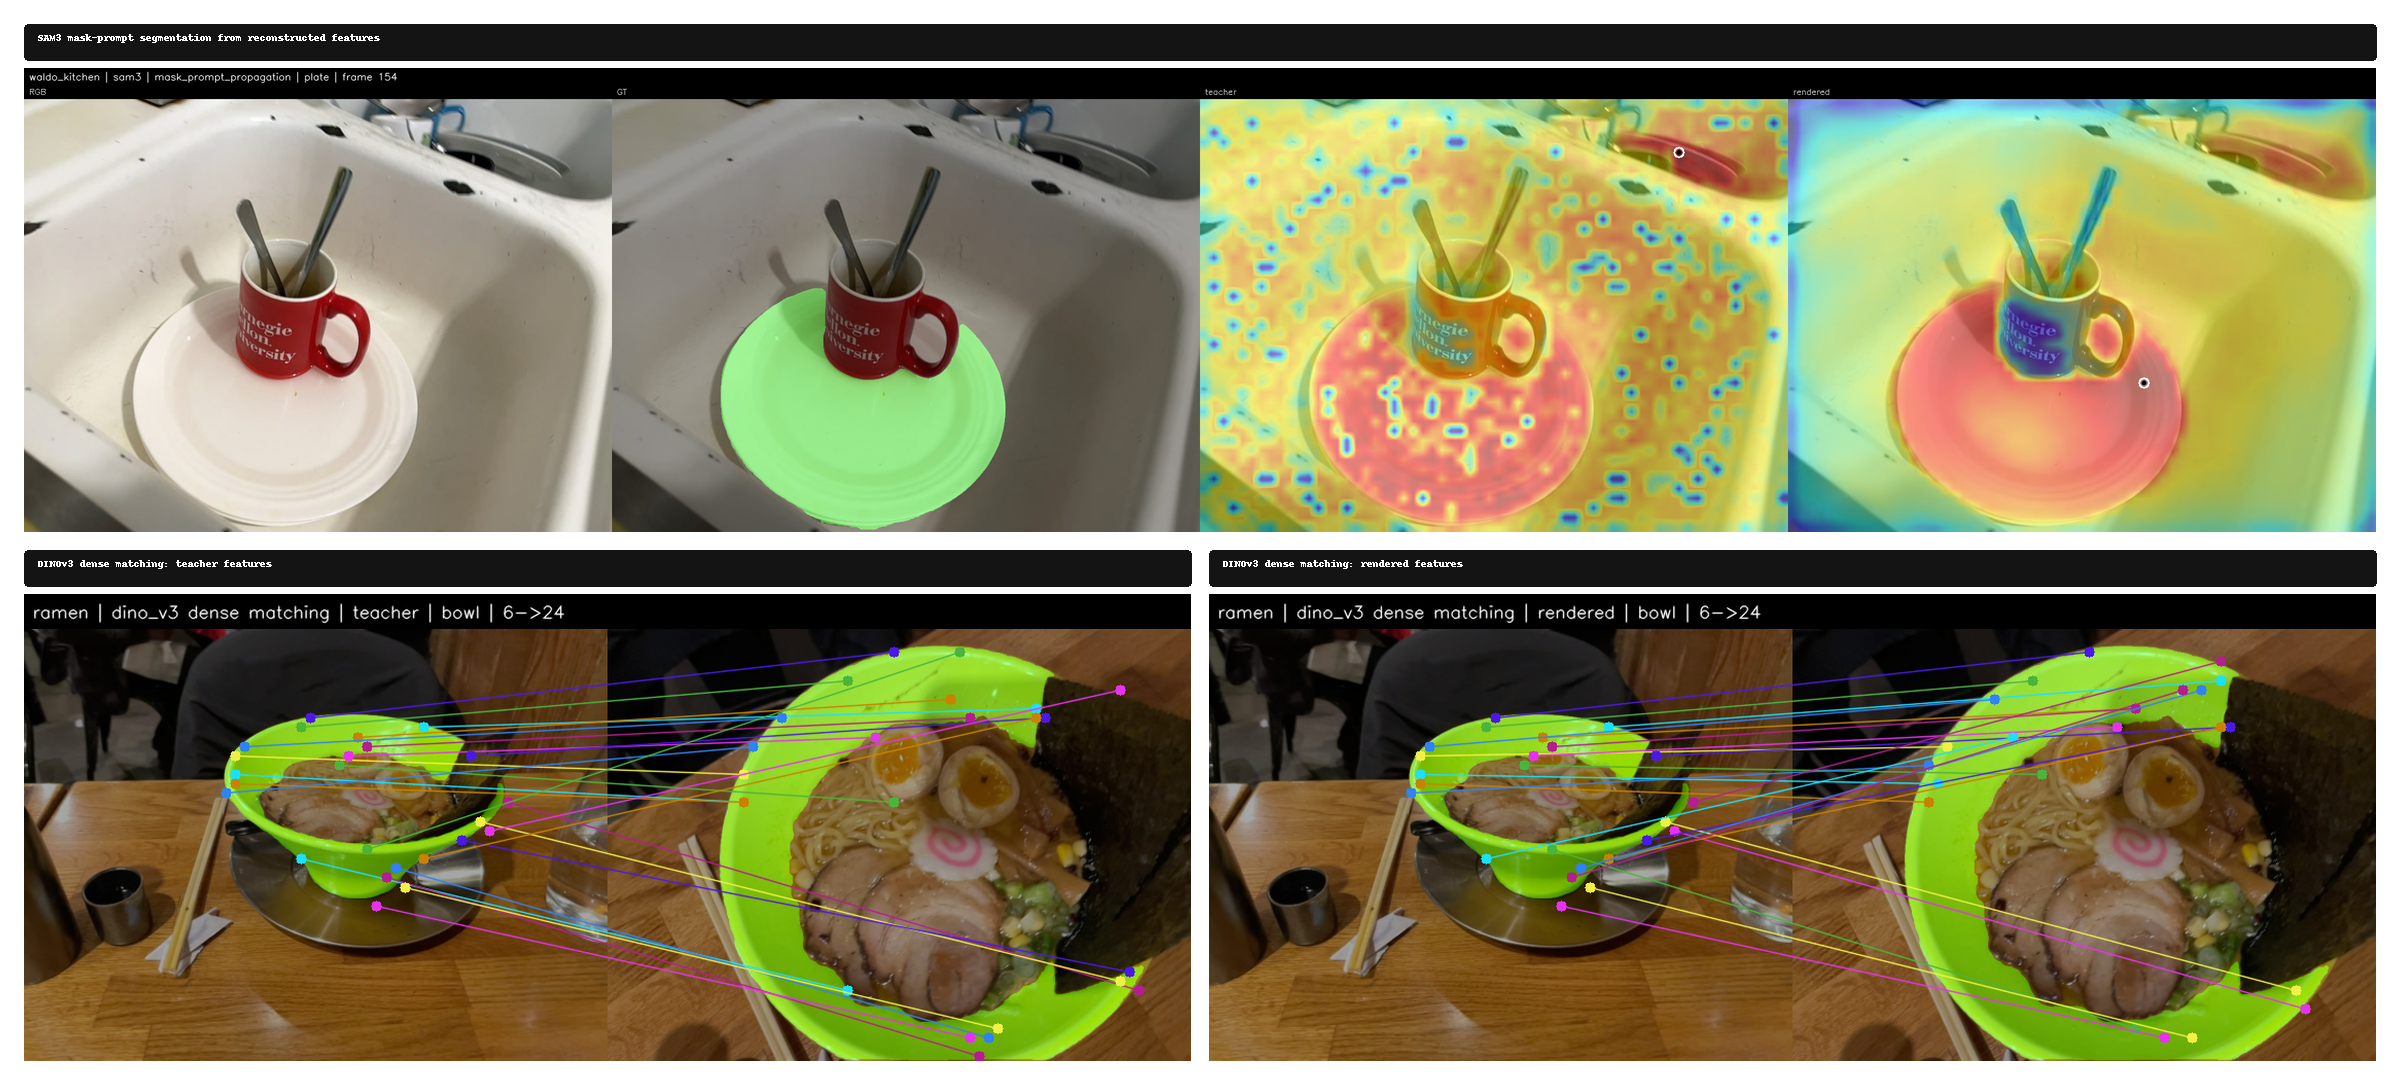
\includegraphics[width=\linewidth]{figures/lerf_sam_dino_tasks_qualitative.png}
\caption{Qualitative promptable downstream probes from reconstructed features.
Top: SAM3 mask-prompt propagation from a source annotation to a target view.
Bottom: DINOv3 source-mask propagation with the promoted background-suppressed
readout. Dense correspondences and homography-RANSAC filtering are kept as
diagnostic visualizations rather than the main quantitative DINO evidence.}
\label{fig:sam_dino_tasks_qual}
\end{figure*}

\subsection{Failure Analysis}

\begin{table}[t]
\centering
\caption{Representative fragile LERF-OVS categories from the frozen rendered-feature evaluation. Low LocAcc with nonzero mIoU highlights the peak-vs-region trade-off.}
\label{tab:failure_analysis}
\begin{tabular}{llrr}
\toprule
Scene & Category & LocAcc & mIoU \\
\midrule
Figurines & bag & 0.00 & 0.00 \\
Figurines & miffy & 0.00 & 0.01 \\
Teatime & dall-e brand & 0.00 & 0.01 \\
Figurines & jake & 0.00 & 0.02 \\
Waldo Kitchen & ketchup & 0.00 & 0.03 \\
Waldo Kitchen & spatula & 0.00 & 0.03 \\
Ramen & corn & 0.00 & 0.10 \\
Figurines & red toy chair & 0.00 & 0.13 \\
\bottomrule
\end{tabular}
\end{table}


Table~\ref{tab:failure_analysis} turns the qualitative small-object observation
into a paper-facing diagnostic. The lowest-ranked categories are mostly tiny or
visually ambiguous objects, such as Figurines bags, character toys, and isolated
kitchen tools. The failure pattern is not only low region overlap: some
categories show nonzero mIoU but zero or partial LocAcc, which means the
rendered heatmap covers a plausible object region while the single maximum lands
outside the annotated polygon. This is why the paper treats mIoU improvements
from adaptor or cross-view losses conservatively unless localization accuracy is
preserved.

\section{Discussion}

\paragraph{Why feature reconstruction matters.}
The LERF-OVS results show that rendered RADIO-like features retain enough
semantic structure for open-vocabulary localization. The ScanNet results suggest
that the same representation can be probed outside the LERF object-query setting.
The LERF direct-selection experiment further clarifies the boundary of this
claim: the compact field supports direct primitive querying once rendered
features are registered back to Gaussians, but the current score-threshold
selection is still weaker than explicit instance- or super-Gaussian grouping on
fragmented scenes.

\paragraph{External-baseline scope.}
The LERF, LangSplat, and LEGaussians comparison rows are now traced to official
paper or supplementary tables. They still come from cross-paper protocols, so
the paper treats them as source-anchored context rows. A strict SOTA claim would
require rerunning those baselines under the same evaluator and annotations used
by \project{}.

\section{Limitations}

\method{} depends on a pretrained Gaussian geometry backbone and does not claim
to improve RGB reconstruction. Small objects remain challenging because the
teacher feature resolution and rendered feature alignment limit heatmap
sharpness. The current ScanNet protocol is a direct point-query feature probe,
not a replacement for a full standardized segmentation benchmark. The registered
LERF direct 3D object-selection readout substantially improves primitive querying
and slightly exceeds the OpenGaussian official macro reference under the reported
OpenGaussian-style context, but it remains weaker on Waldo Kitchen and is not a
locally rerun same-evaluator comparison. The paper should therefore avoid
claiming universal primitive-level SOTA. Confidence-weighted VPR-to-field
consistency improves the direct student field substantially, but it does not
yet fully replace the streamed registered VPR readout on all scenes. Finally,
the external comparison is official-source but not reproduced under one evaluator, so
strong SOTA-style claims require additional baseline reruns. The storage table
reports checkpoint footprint rather than a deployed runtime memory allocator, so
future packaging should separate feature-field parameters, rendering buffers, and
optional downstream heads.
The training entry point is now a modularized release artifact: the
reproducibility audit verifies manifest, split, trusted-checkpoint,
metrics-history, training-lock, and wrapped tensor-cache guards, and the
entry script is reduced to 3735 lines with support code under
\texttt{radio\_gs/training}.

\section{Conclusion}

\method{} turns a 3D Gaussian scene into a reusable foundation-feature memory.
By reconstructing frozen RADIO features rather than training a scene-specific
classifier, it supports open-vocabulary grounding and cross-domain feature
queries from novel views. The current freeze package provides a coherent
submission path: strong LERF-OVS internal results, fair ScanNet direct-query
evidence, explicit storage and runtime profiles, failure analysis, and
source-anchored external comparison caveats.

\bibliographystyle{ieeenat_fullname}
\bibliography{radio_gs_refs}

\end{document}
